\chapter{Model and System Design}
\label{chap:methodology}

This chapter details our model implementation and system design. In Data Collection, we list the sources of our font file data as well as our methods for data handling. Our Models section describes the design of our three autoencoder-based models: the Basic Autoencoder model, Style Transfer model, and a more sophisticated model adapted from Srivatsan et al.\ \cite{srivatsan2020}. Finally, in the System Design section, we discuss our considerations in building a font selection tool based around our model style encodings, and we explain the design of our final implementation: a font selection interface which navigates high-dimensional typeface style space.

\section{Data Collection} \label{data-collection}

In order to train models to effectively encode the style of typefaces, it was necessary to create a dataset of characters from a wide variety of fonts. Given the stylistic diversity between fonts, it was important that the dataset be large and representative enough to encompass the variety of existing typeface styles---so that the model would work effectively not just for fonts in its training set, but for unseen fonts as well.

The first important consideration was the source of our data. The model proposed by Srivatsan et al.\ \cite{srivatsan2020} was trained on the large Capitals64 dataset constructed by Azadi et al.\ \cite{azadi2017}. We also chose to use this dataset, but opted to add some additional sources of fonts. Specifically, we included the entire library of fonts from the Google Fonts repository,\footnote{\url{https://github.com/google/fonts/}} which contains a wide range of free-to-use fonts, and we also included the default fonts which come preinstalled with macOS (which contains many of the well-known proprietary fonts not represented in Google Fonts or Capitals64). In the latter two cases, we only considered fonts which supported English-language text, choosing to ignore typefaces in other scripts (Chinese, Arabic, Bengali, e.g.) for the scope of this research. Ultimately, we included in our dataset 10,682 typefaces from the Capitals64 dataset, 3,577 from Google Fonts, and 132 fonts from the installation of macOS. We felt that this combined dataset ($n = 14,391$) would be both sufficiently large and representative of a wide variety of typeface styles, while still containing well-known proprietary fonts such as Times New Roman and Helvetica.

The fonts we sourced came as TrueType (.ttf) and OpenType (.otf) binary font files, both of which contain the raw data for individual typefaces or multiple typefaces in one family (Helvetica and Helvetica Light, e.g.). We used the open-source FontForge scripting package\footnote{\url{https://fontforge.org/en-US/}} to create an SVG vector image file for each character represented in each typeface, then rasterized the character vector files to $64 \times 64$ pixel images in PNG format. We additionally created $1664 \times 64$ images representing the 26 capital letters (A-Z) in each typeface to fit the Capital64 data format expected by the Srivatsan et al.\ model implementation. For font files which contained multiple styles in a given font family (e.g.\ Times, Times Italic, and Times Bold), we treated each style as a separate typeface, since their respective style representations should be meaningfully different.

\section{Models}

Over the course of our research, we employed several model training methods. This section details the various approaches and their respective model architectures. All models were trained using PyTorch 2.5.1 and Python 3.13 running on a Bizon G7000 G2 GPU server with 2x 32-Core 2.00 GHz Intel Xeon Gold 6338 CPUs and 4x NVIDIA RTX A6000 48 GB GPUs. Generally, we trained our models until the model loss plateaued, i.e. the font reconstruction task stopped improving.

% my own figure
\begin{figure}[]
    \centering
    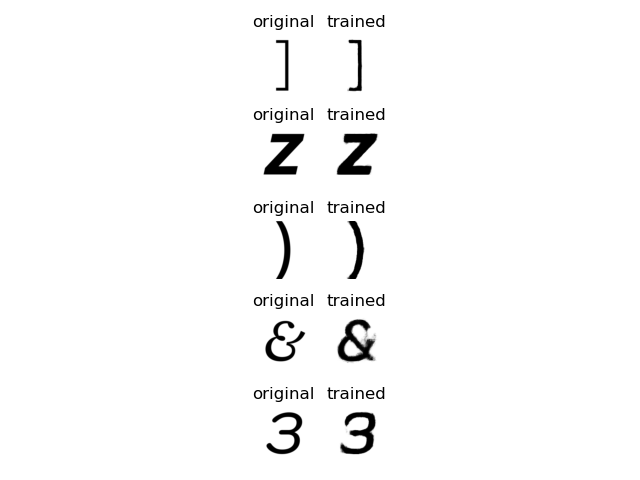
\includegraphics[width=\textwidth]{images/autoencoder-example.png}
    \caption{Our basic autoencoder model inputs/outputs mid-way through training}
    \label{fig:autoencoder-example}
\end{figure}

\subsection{Basic Autoencoder} \label{basic-autoencoder-2}

For our first approach, we adapted the autoencoder model proposed in \cite{rumelhart1986}. As previously explained, an autoencoder is a neural network trained to compress and reconstruct input data. By doing so, it can learn to generate meaningful encodings of input data; in the case of our research, we hoped to capture typeface style in these model encodings. We implemented an autoencoder model trained on our large dataset of font character images, represented as pixel-intensity matrices. Our model uses a series of alternating linear layers and ReLU activation functions to compress the $64 \times 64$ pixel images (flattened to length-4096 vectors) down to length-6 vectors, approximately halving the size of the vector with each linear layer. The decoder, conversely, expands the representation back to its original size with a series of linear and non-linear layers, ultimately converting the vectors back into $64 \times 64$ pixel intensity matrices. To compute the loss of our model, we used mean squared error (MSE) between respective pixel values in the input and output matrices. After computing this loss, we translated the pixel intensity matrices back into their original image form, in order to visually evaluate the success of our reconstructions.

% my own figure
\begin{figure}[]
    \centering
    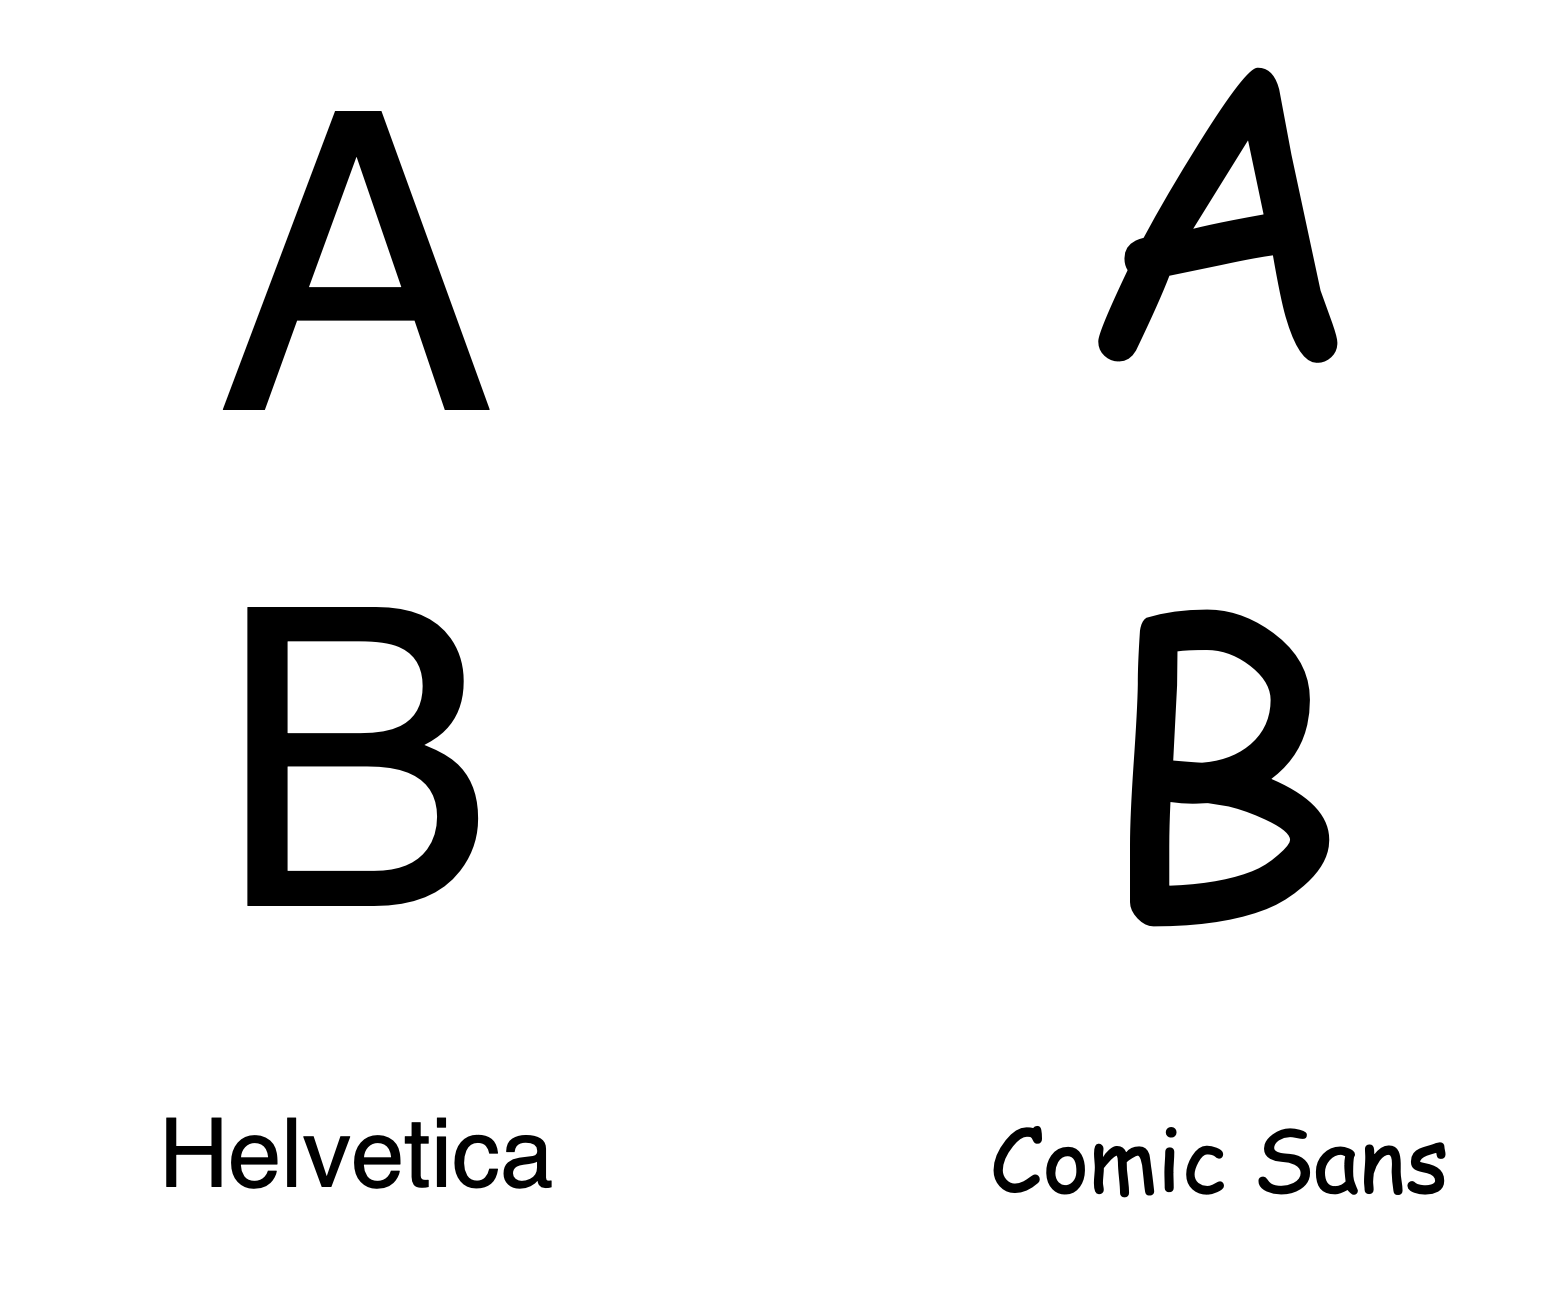
\includegraphics[width=0.55\textwidth]{images/ab-cs-helvetica.png}
    \caption{An {\fontspec{Helvetica} A} in Helvetica is structurally more similar to an {\fontspec{comicsans.ttf} A} in Comic Sans than to a {\fontspec{Helvetica} B} in Helvetica}
    \label{fig:ab-cs-helvetica}
\end{figure}

Some example input and output from our initial autoencoder model can be found in Figure \ref{fig:autoencoder-example}. Even early in the training, the model was able to accurately reconstruct most of the input characters, although it struggled more with more complicated typeface styles. However, we quickly identified an issue with this model: the autoencoder has no obvious incentive to distinguish form (the style of a character, defined by its font) from content (the actual letter which is represented). For example, an {\fontspec{Helvetica} A} in Helvetica looks substantively different from an {\fontspec{comicsans.ttf} A} in Comic Sans, but an {\fontspec{Helvetica} A} in Helvetica \textit{also} looks substantively different from a {\fontspec{Helvetica} B} in Helvetica, simply because they are different letters. In fact, the Helvetica {\fontspec{Helvetica} A} is structurally \emph{more} similar to the Comic Sans {\fontspec{comicsans.ttf} A} than the Helvetica {\fontspec{Helvetica} B} (see Figure \ref{fig:ab-cs-helvetica}). Our basic autoencoder does not have sufficient information to decouple the stylistic similarity of Helvetica's {\fontspec{Helvetica} A} and {\fontspec{Helvetica} B} from the structural similarity of the the Comic Sans {\fontspec{comicsans.ttf} A} and the {\fontspec{Helvetica} A} in Helvetica. Under this model, the dimensions of the resulting style encoding likely conflate variance in style with variance in the characters themselves.

In order to create style encodings for style-based font selection, an effective model must be able to understand \emph{character} as separate from \emph{style.} Characters in the same font should all be understood to have one style, determined by the font itself, while two characters in different fonts should have different style encodings (which might be more or less similar depending on their respective styles).

\subsection{Style Transfer Autoencoder} \label{style-transfer}

% my own figure
\begin{figure}[]
    \centering
    \includegraphics[width=\textwidth]{images/style-transfer-model.pdf}
    \caption{Our Style Transfer Autoencoder model, which attempts to recreate a different character in the typeface of an input character image}
    \label{fig:style-transfer-model}
\end{figure}

To disentangle style from character, we trained a modified autoencoder on a different task: to recreate \textit{other} characters in a given font. For example, given an input image of a C character, we trained the model to output a Q character in that same font. In order to provide the necessary information for the model to succeed in this task, we included two additional vectors in the model input: one representing the character of the input image, and the other representing the target character. Figure \ref{fig:style-transfer-model} illustrates this schema. The model takes as input a characer image, along with the vector embedding parameter representing the character information, and additionally takes the target character embedding as a mid-way input to provide the decoding step with the requisite information to construct the target image. By minimizing the MSE between the generated character (say, a {\fontspec{Arial} Q} in Arial) and the ground truth image in our dataset, we hypothesized that our model would better isolate style in its encodings. The model has no need to represent character in the intermediate encoding, since both the encoder and decoder explicitly receive auxiliary character information. 

The inclusion of auxiliary input vectors required that there be a fixed-size character set. We originally experimented with limiting our training data to only include fonts which contained all uppercase (A--Z) and lowercase (a--z) English characters; however, in order to incorporate the Capitals64 dataset---which only includes capital letters---we decided to limit our training only to fonts including the English uppercase letters. Fonts which did not contain the 26 uppercase letters A--Z were excluded from training.

For the style transfer model, we had to modify the data loading process. Rather than dealing with every individual character in a font, we needed to handle every \textit{pair} of characters in a font. Since we were considering 26 characters per font, our model trained on ${}_{26}C_2 =$ 325 character pairs per typeface. Additionally, since we were considering the input/output characters as data inside our model, unlike the basic autoencoder approach, we also created embeddings for each of the characters within our model architecture. The input embedding was concatenated with the flattened input image before it was fed to the encoder, and the output character embedding was concatenated with the intermediate vector representation between the encoder and decoder. Finally, we computed the MSE loss not against the input image but against the ground truth goal image representing the target character in the selected font.

Figure \ref{fig:styletransfer-example} shows our style transfer model part-way through training. The model receives the input {\fontspec{kumar-one.ttf} B} glyph and the input/output character embeddings (not shown), and it attempts to reconstruct the {\fontspec{kumar-one.ttf} h} glyph in the same typeface. By giving the model explicit vector representations of the input/output characters, we hypothesized that the model would more effectively isolate the style of the glyphs as separate from their content, giving us better internal representations to leverage for style-based typeface selection.

\subsection{Srivatsan Model}

% my own figure
\begin{figure}[]
    \centering
    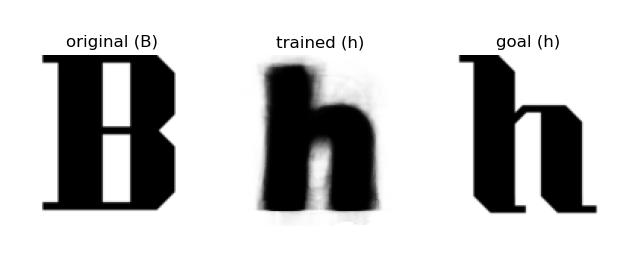
\includegraphics[width=\textwidth]{images/styletransfer-example.png}
    \caption{Example instance of our style transfer model part-way through training}
    \label{fig:styletransfer-example}
\end{figure}

Our final model, which we adapted from Srivatsan et al.\ \cite{srivatsan2020}, mirrors our previous approaches in many ways, but it introduces several techniques hypothesized to improve the stylistic encoding ability of the model on our dataset. Most notably, the Srivatsan model incorporates variational inference and convolution. It may be necessary to define these terms: a variational encoder, rather than explicitly encoding an intermediate vector representation between the encoder and decoder steps, produces intermediate parameters $\mu$ and $\sigma$ of a multi-dimensional Gaussian distribution, from which a vector representation is randomly sampled and then decoded. Proposed by Kingma et al.\ \cite{kingma2019}, variational autoencoders (VAEs) are often used for generative tasks in deep learning, as they represent a large probabilistic space of outcomes. However, even in non-generative tasks such as ours, the variational model can generate useful, often more stable model encoding spaces.

Convolution, and convolutional layers---a technique which is separate from variational modeling but can be used in tandem with that technique, as in the case of the Srivatsan model---involves a moving filter called a kernel which reduces spatial dimension. In the case of typeface style encoding, this dissociates style elements from their particular location in training images. For example, the serif elements of characters in a serif typeface (i.e. the tail at the ends of characters like T and S) appear at many different locations in a training image depending on the particular character and typeface; using convolutional layers allows the model to recognize these elements regardless of their specific location in an image. Therefore, the model better identifies serif elements across many different characters, locations in those characters, and serif typefaces.

% my own figure
\begin{figure}[]
    \centering
    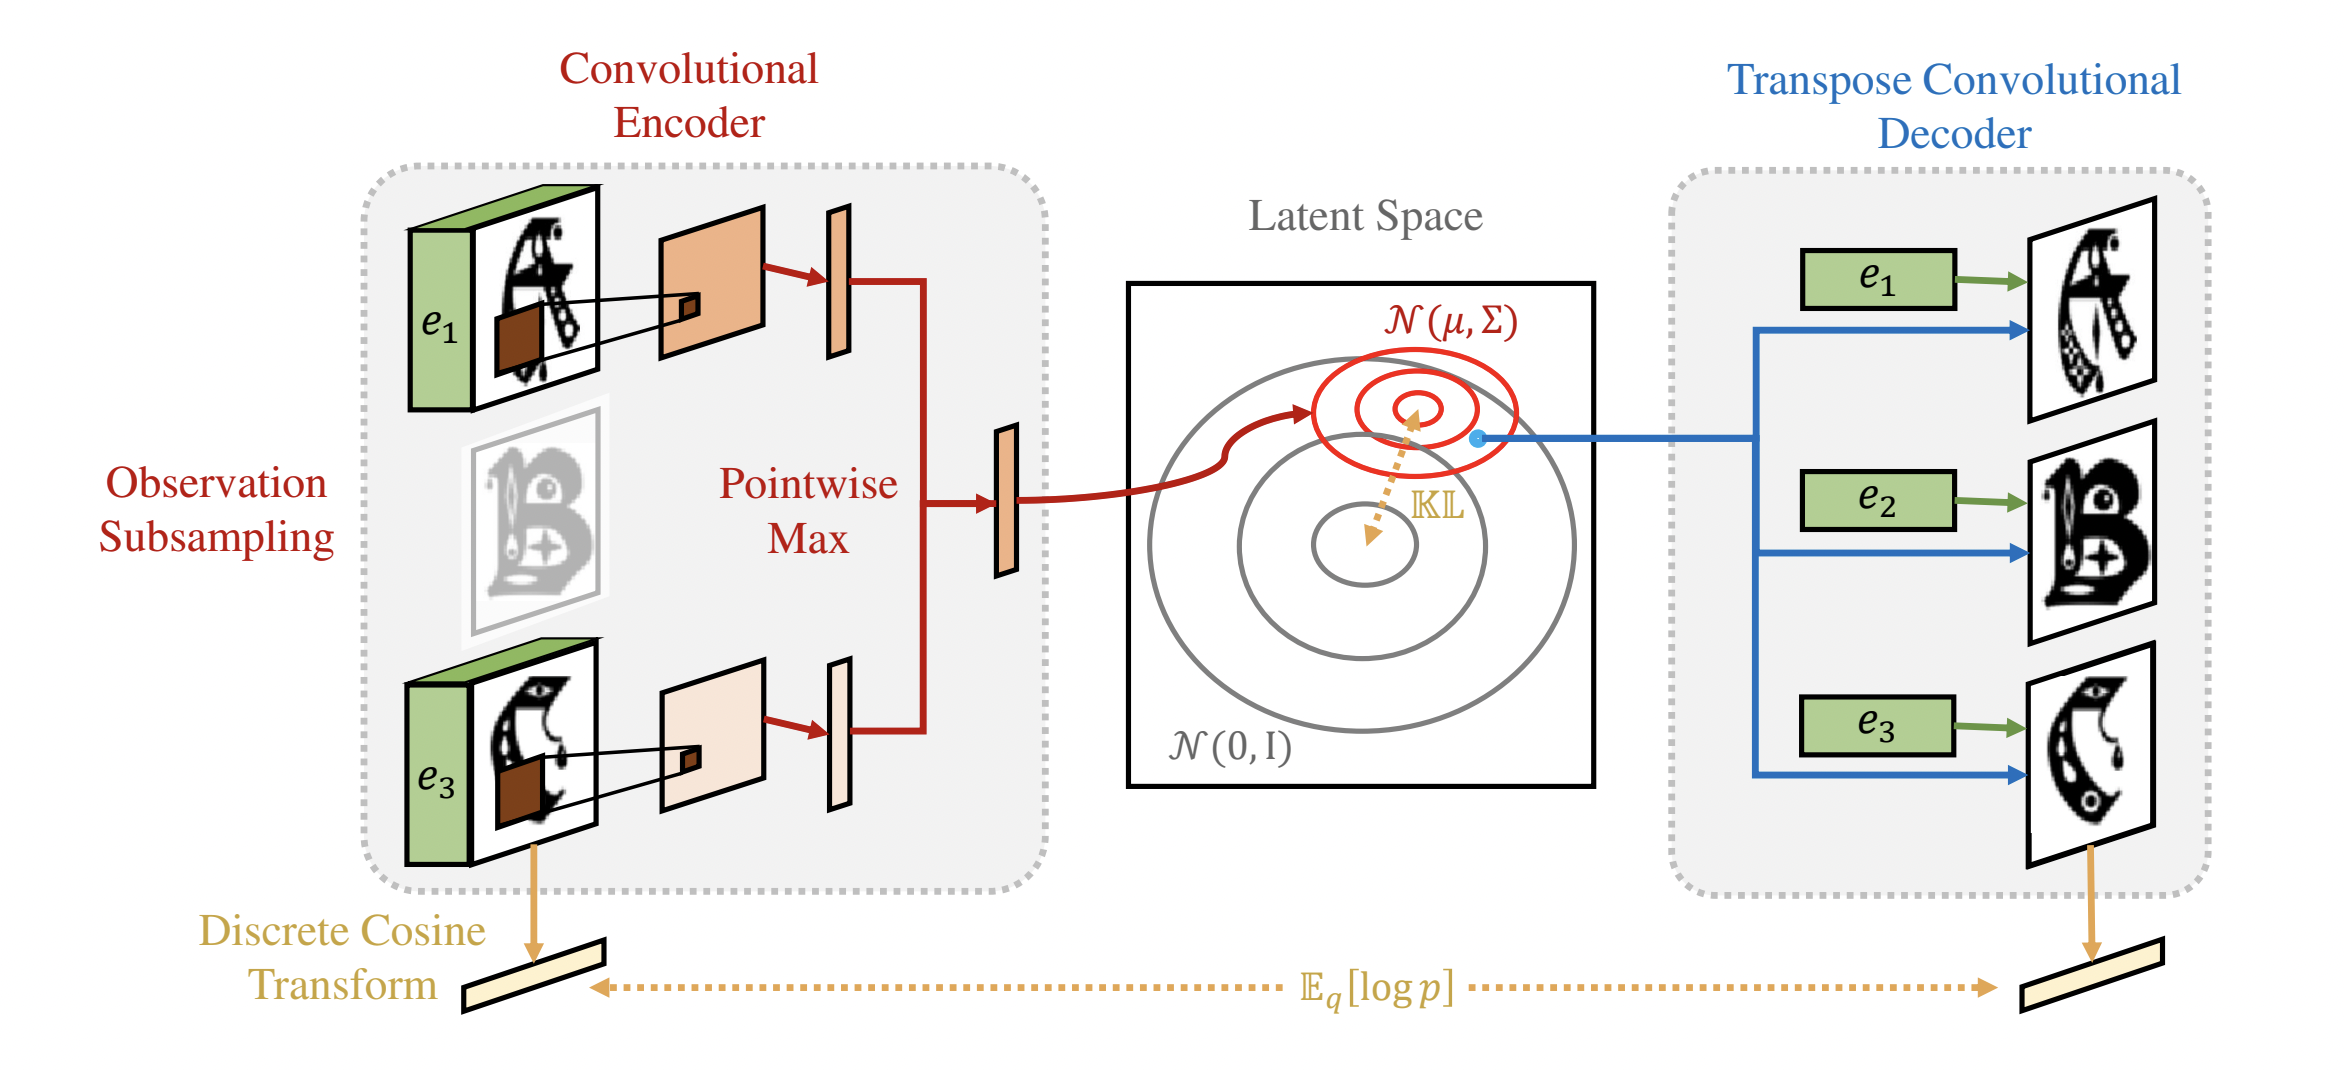
\includegraphics[width=\textwidth]{images/srivatsan-model.png}
    \caption{Diagram of Srivatsan et al.\ model architecture \cite{srivatsan2020}}
    \label{fig:srivatsan-model-2}
\end{figure}

Lastly, the Srivatsan model approaches style encoding using a slightly different task: it includes a full set of characters as input data for character reconstruction, and it approaches the character reconstruction task across an entire typeface at once---rather than reconstructing each character or character pair individually. Similar to our Style Transfer model detailed in \ref{style-transfer}, the Srivatsan model aims at recreating different characters across a typeface and involves vector character embeddings for those input/output characters; however, the model takes the full set of uppercase characters A--Z and randomly masks a set number of characters for reconstruction, rather than dealing with characters individually. The model reconstructs the missing characters based on the given (non-hidden) characters in the font, as well as the character embedding information for the hidden characters. The encoder creates a Gaussian encoding from the input, and the decoder uses that encoding along with the respective respective character embedding for the masked glyphs to reconstruct the full character set for a given typeface. The model also applies a 2-Dimensional Discrete Cosine Transform (2-D DCT-II) \cite{ahmed1974} to the generated images before computing the loss, with the goal of generating sharper images. DCT-II is simply a rotation in vector space, meaning the resulting probability measurements and vector distances are preserved. A diagram of the Srivatsan model architecture can be found in Figure \ref{fig:srivatsan-model-2}.
 
The Srivatsan model does an adequate job at glyph reconstruction---one of the focuses of the paper---but also generates promising style encodings. Figure \ref{fig:srivatsan-tsne} shows a t-SNE \cite{vandermaaten2008} plot of the latent style encodings generated by the Srivatsan model, colored by both weight and Google Font style category. As the figure shows, it is quite effective at clustering fonts with similar weight (bolder or lighter) and more ambiguous stylistic aspects provided as metadata with Google Fonts.

% my own figure
\begin{figure}[]
    \centering
    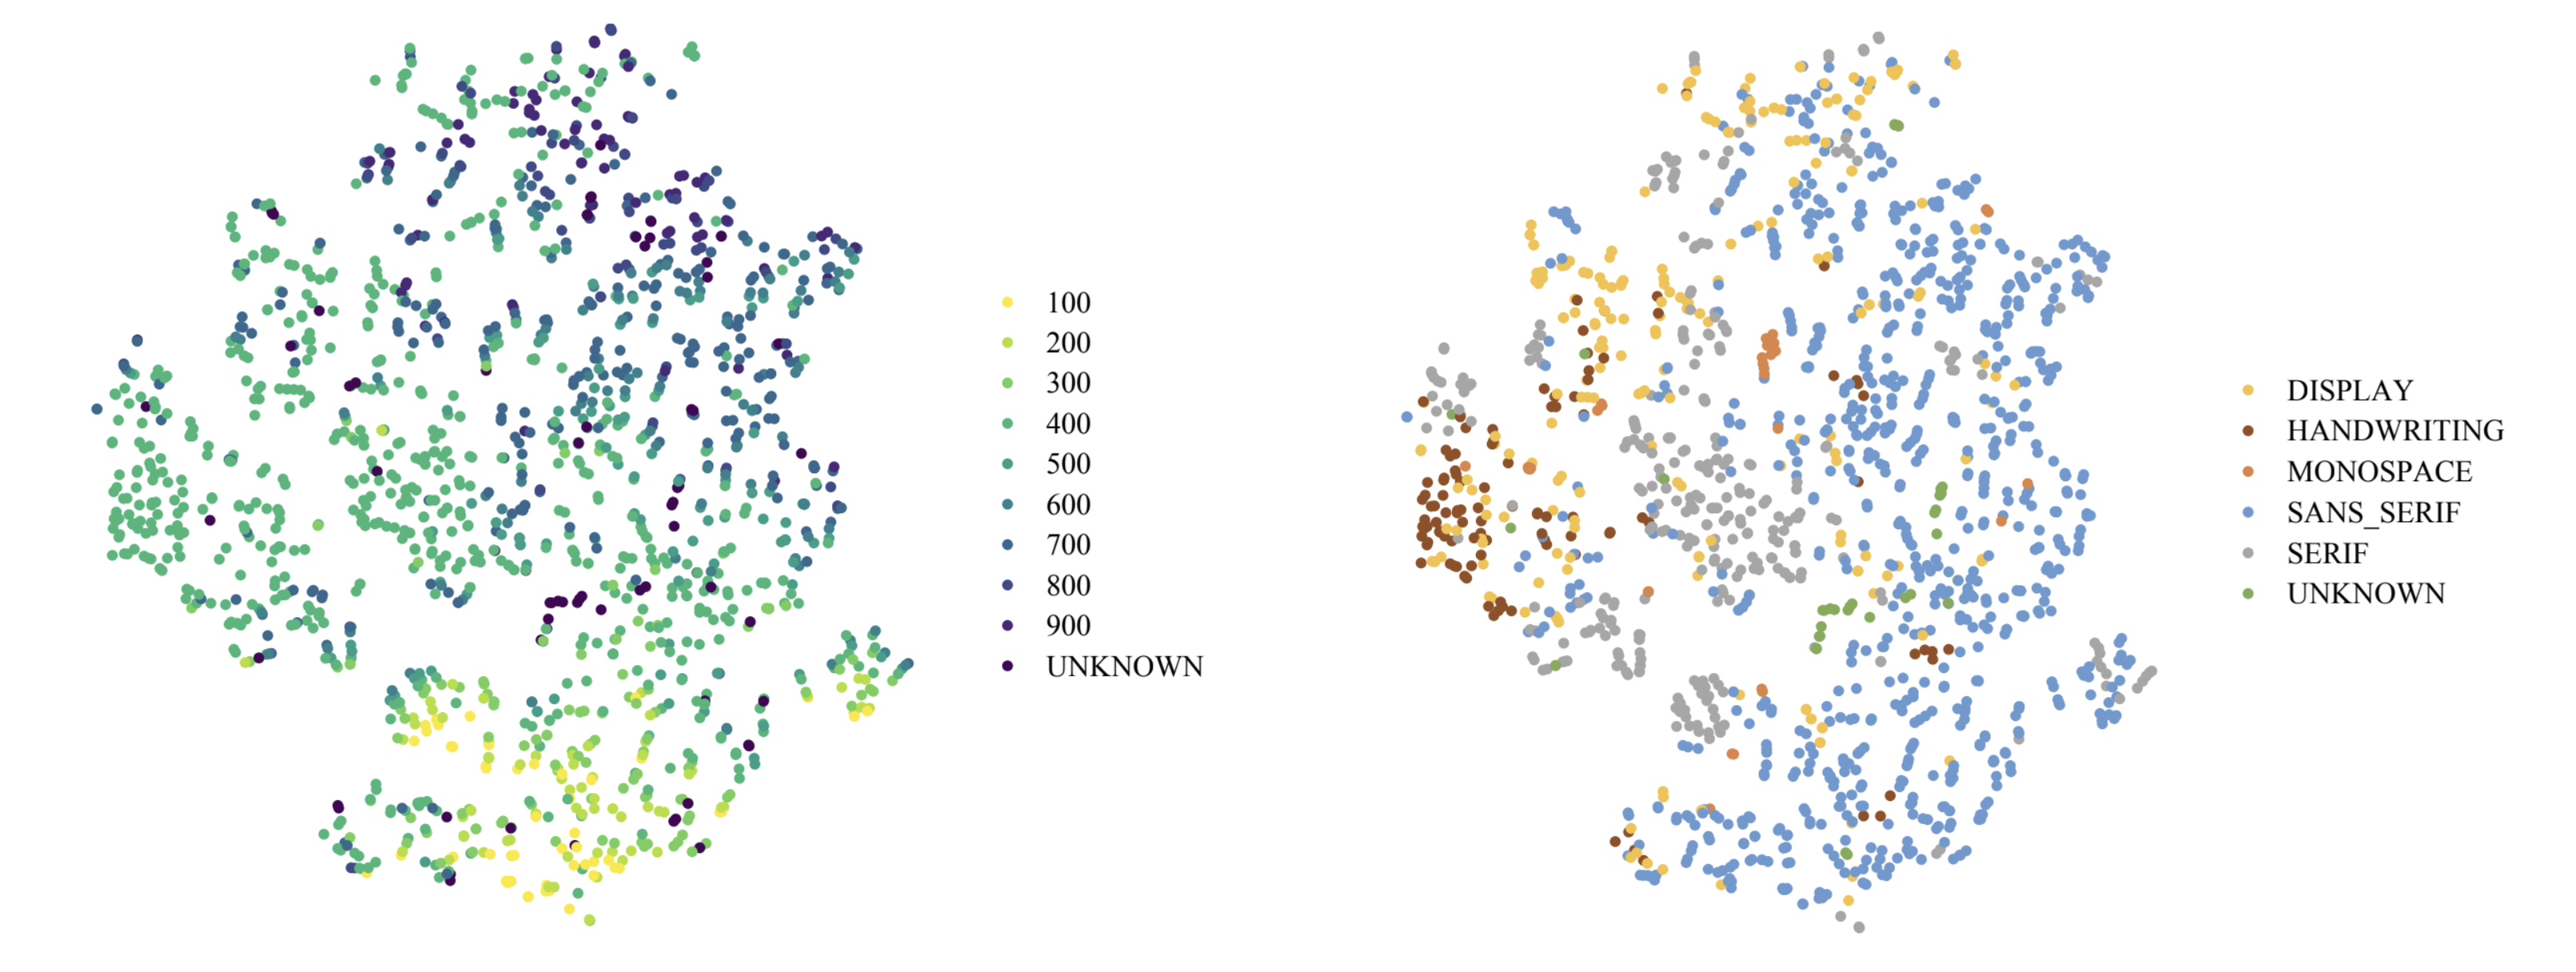
\includegraphics[width=\textwidth]{images/srivatsan-tsne.png}
    \caption{t-SNE plot of style encodings from Srivatsan et al.\ \cite{srivatsan2020} colored by weight (left) and Google Fonts style category (right)}
    \label{fig:srivatsan-tsne}
\end{figure}

We ported the original code from Srivatsan et al.\ \cite{srivatsan2020} from Python 2.7 and PyTorch 1.1.0 to Python 3.13 and PyTorch 2.5.1 and trained it on our extended dataset, with 10 hidden characters per font, for 184 epochs. After training, we ran the model on a modified version of our Google Fonts dataset in order to generate useful style encodings which we could compare against our other models and use in our webapp font selector tool. As with our other models, we trained the modified Srivatsan model until the MSE loss plateaued and the model seemed (by visual inspection) to adequately reconstruct the missing characters for most input character sets.

Figure \ref{fig:srivatsan-reconstructions} shows 44 reconstructed character sets from the Srivatsan model, with 10 characters per typeface randomly masked and reconstructed by the model. The model seems better at reconstructing some fonts than others---specifically, it seems to have performed better on typefaces with more common styles, such as basic serif or sans-serif fonts. Stranger, more uncommon font styles were not reconstructed as accurately (for example, the third font from left in Figure \ref{fig:srivatsan-reconstructions}). However, character reconstruction is not out primary objective. Our main goal is to encode typeface style using the intermediate representation of the model, which does not correspond exactly with the model's character reconstruction ability. Nevertheless, the highly accurate reconstruction performance we see for many of the typefaces, along with a somewhat-decent reconstruction of the more difficult fonts, suggests a fairly strong representation of typeface style within the model. Further evaluations in Chapter \ref{chap:evaluation} quantitatively analyze the style-encoding capabilities of our three models.

% my own figure
\begin{figure}[]
    \centering
    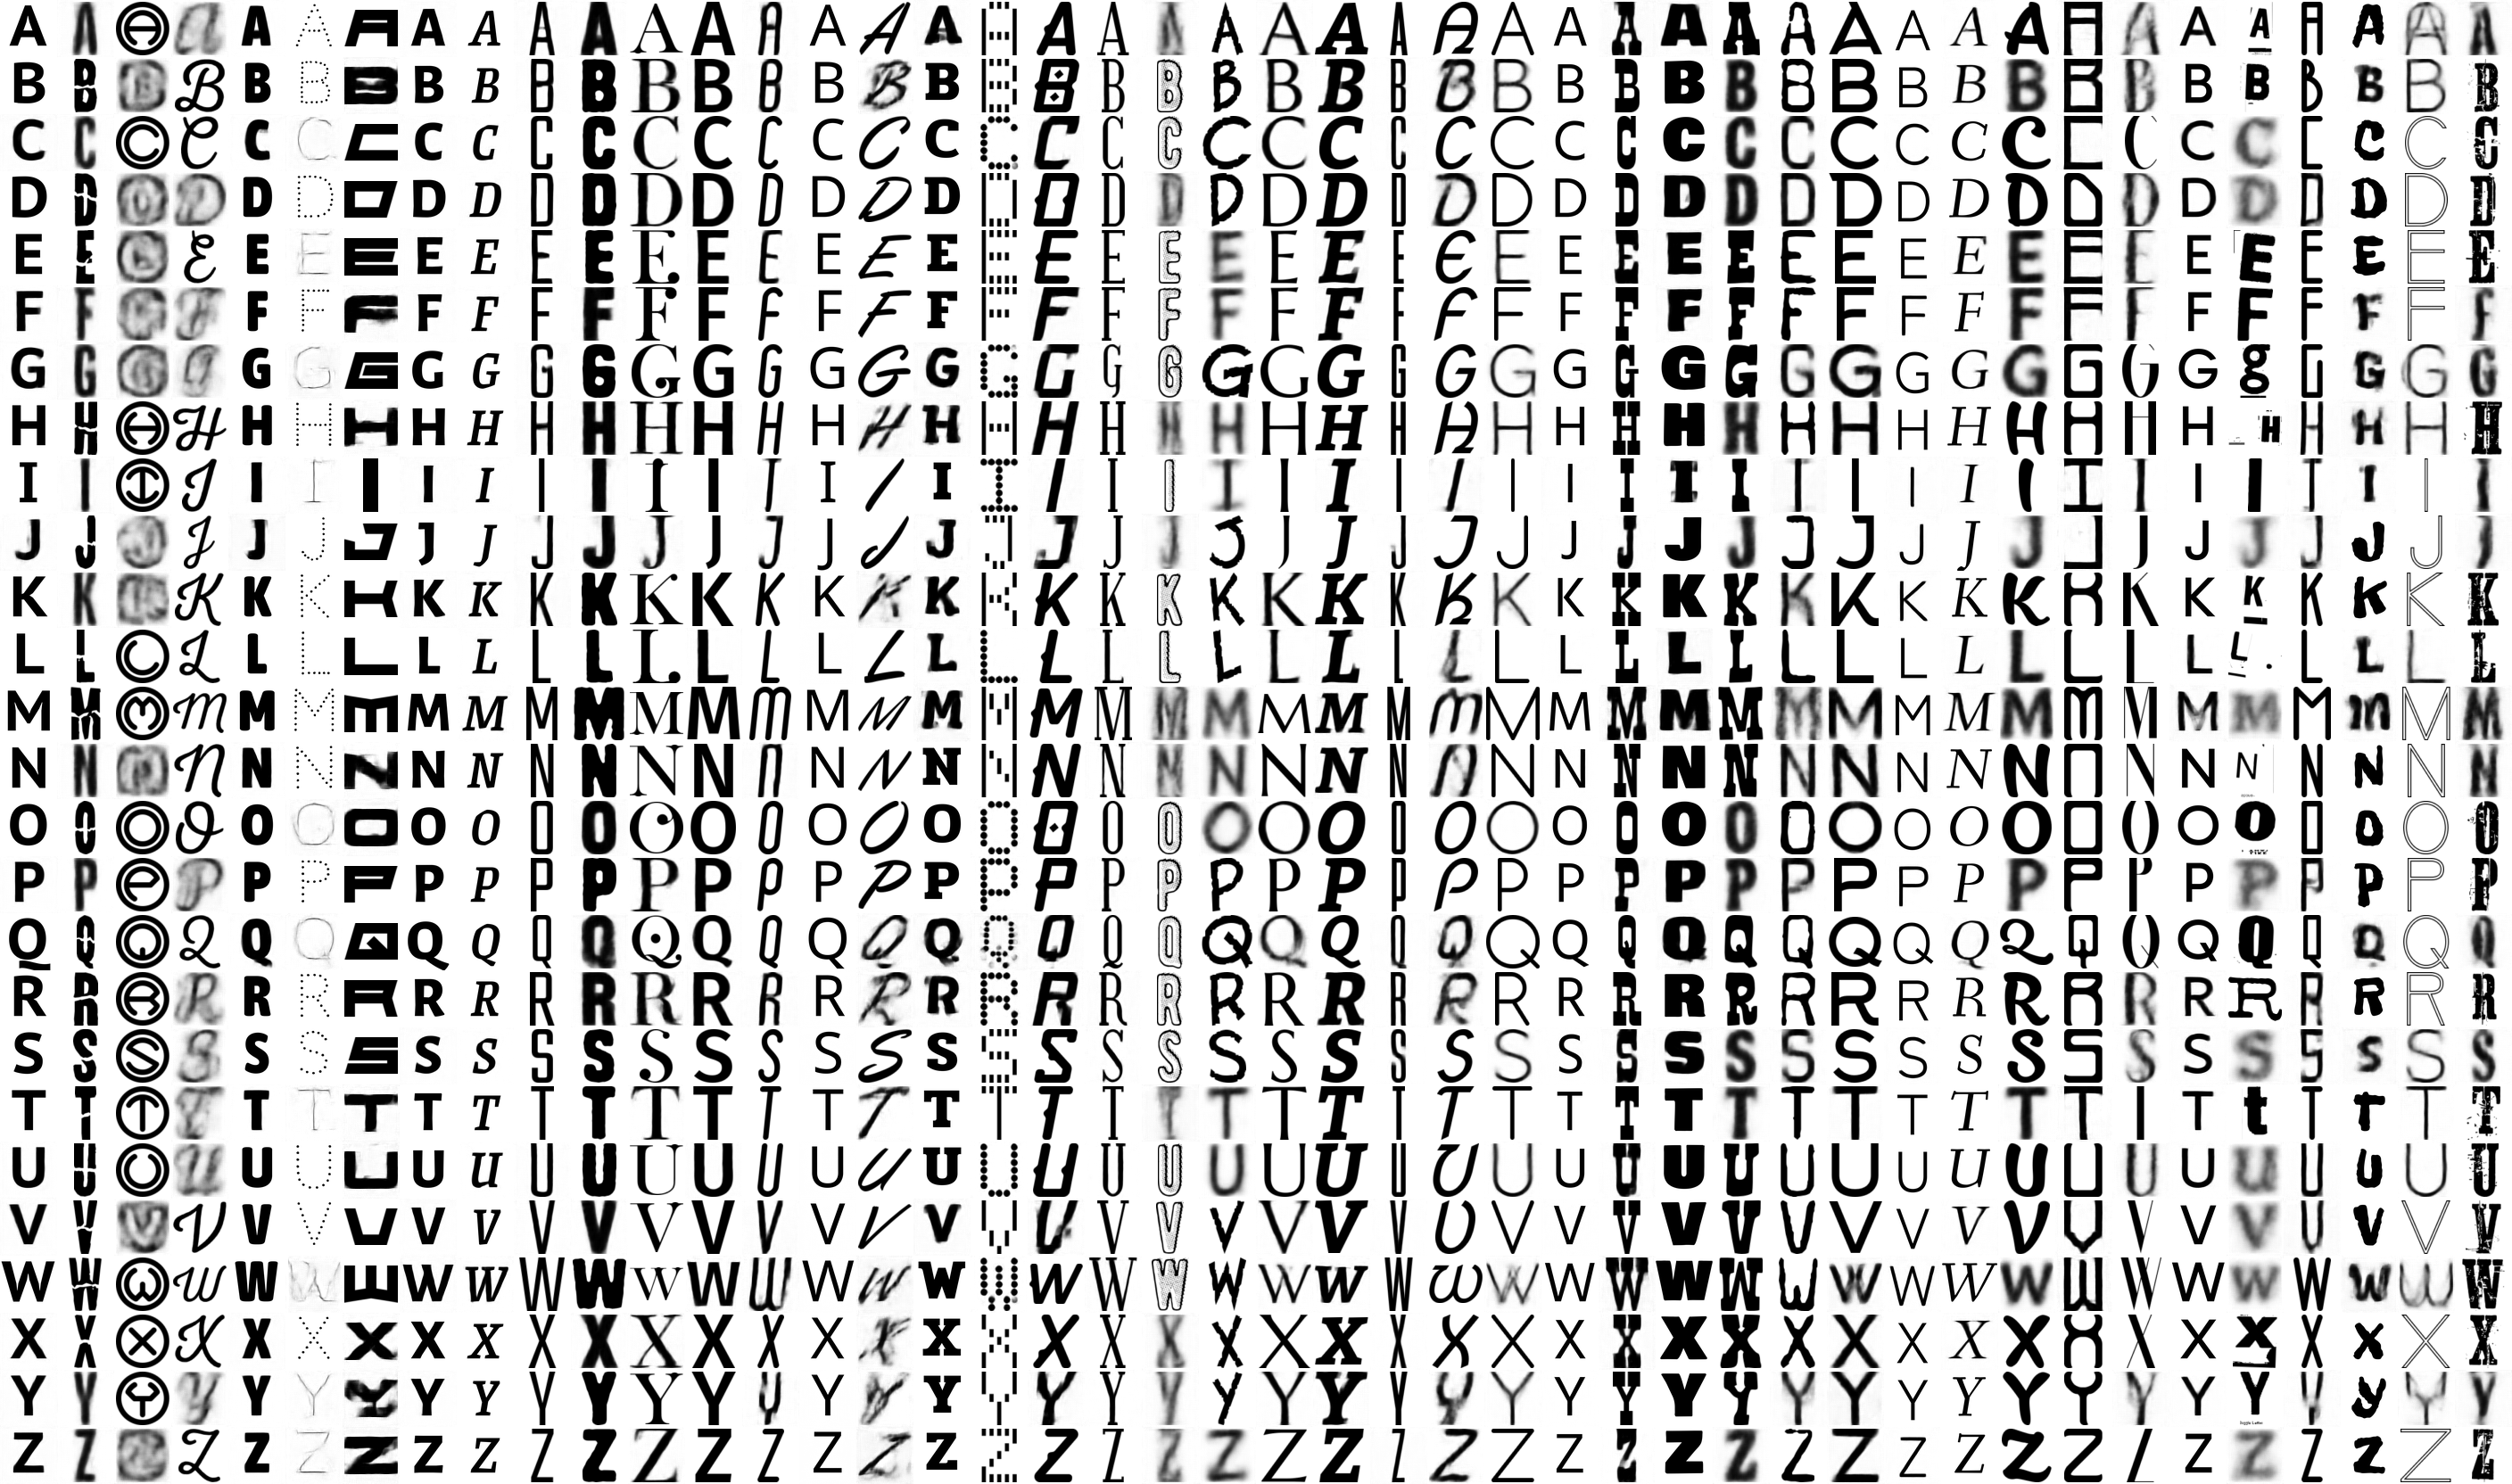
\includegraphics[width=\textwidth]{images/srivatsan-reconstructions.png}
    \caption{Reconstructed character sets from the adapted Srivatsan model}
    \label{fig:srivatsan-reconstructions}
\end{figure}

\subsection{Extracting Style Encodings}

In order to build useful typeface selection tools based on these models, it was necessary in all three cases to extract the model's internal style encoding vector for each typeface. This task was relatively trivial for the first two models: we simply passed each of the typeface character sets through the encoder portion of our model and performed an elementwise average across the resulting vector representation for each character, which we believed would generate a roughly-representative style encoding for the entire typeface. For the Srivatsan model, we similarly ran our model on each of the typeface character sets; however, since the Srivatsan model applies a variational approach, it was additionally necessary to perform a random sample from the Gaussian distribution defined by each typeface character set to obtain a style encoding. Because the architecture of the Srivatsan model does not train on individual character sets or pairs, but entire typeface character sets together, it was not necessary to take an average of multiple character style encodings; the model, by design, trains one generalized latent style encoding for each typeface.

\section{System Design}

In this section, we detail the process and design of turning our style encodings—generated by the models in the previous section—into a user tool for typeface selection. We consider questions of encoding dimensionality, end-to-end system design, and user experience in order to create a novel, useful typeface selector tool.

\subsection{Style Encoding Dimensionality}

One initial question which emerges when training autoencoder-like models---especially with the goal of extracting intermediate encoding vectors---is: what should be the dimensionality of those encodings? In our case especially, there is a tradeoff between encoding more information (higher dimensional vectors should be able to represent greater stylistic detail, to a certain point) and usability (lower dimensional vectors represent fewer choices for users, presumably yielding easier-to-use tools). One could, for example, train a model to generate 2-dimensional style encodings; this could yield a very straightforward interface, such as a scatterplot of typefaces or two sliders corresponding to the two style axes, but two dimensions may not have the capacity to represent the many diverse aspects of typeface style. Alternatively, one could choose a high dimensional style encoding—say, a 100-dimensional vector—which would have a greater capacity to encode font style; however, presenting a user with a decision for each of those dimensions would be unwieldly and overwhelming.

We tested several embedding dimensions, but ultimately chose to encode typeface style using 6-dimensional vectors. This provides substantial capacity to represent typeface style, but also reasonably limits user choice. In the following section, we describe how these six dimensions translate to a novel font selection tool; additionally, we compress these 6-dimensional style encodings into 2-dimensional space using t-SNE reduction to create an auxilliary scatterplot tool which provides users with an additional graphical representation of the data.

\subsection{User Experience}

We experimented with several iterations of a tool for intuitively exploring a space of high-dimensional style encodings. As mentioned previously, the question of dimensionality is a significant one when generating style encodings for user interaction; another important consideration is \textit{how} users should interact with these high-dimensional vector spaces. Should users have full control over each dimension, or should they be guided in their decisions? How should high-dimensional space—which cannot be easily visualized or conceptualized by users—be represented? What additional features (a back button, the ability to save a typeface for later reconsideration, a search bar) would help a user navigate this high-dimensional stylistic vector space? Moreover, what is the goal of our user (finding a specific font, finding similar fonts to a given font, or open exploration)? How much time is the user willing to spend searching for a font? What does the user want to do with this font (or fonts) once identified, and how can we assist the user to accomplish that? We hoped to design a tool that would address these many considerations.

\subsection{Lessons from Early User Tool Implementation}

Early in the development process, we implemented a user tool which included a numerical slider for each dimension of the model space and allowed users to generate new characters based on the model---namely, by inputting the user-determined vector into the model decoder and displaying the output generated character. Our goal was to visualize the dimensions of the model space, to see what sort of information about the characters were being encoded by the model. There were a few issues with our approach: first of all, the interface was inherently a generative task---users would generate new characters/typefaces rather than selecting a preexisting typeface in a dataset---which is a sort of task we later gave up (mostly because the resulting generated typefaces just don't look very good); secondly, this earlier interface was built atop our Basic Autoencoder model, meaning the different dimensions dictated by the sliders would change both style and character at once. Our most important takeaway, however, was that the tool afforded users too much control and not enough guidance while exploring fonts. Even with a relatively low-dimensional space like ours, giving users direct control over several continuous sliders did not make for a very good user experience. Our current interface, while still providing many different methods and dimensions of user control, is a bit more limited and guided with its options, hopefully making for a more useable tool.

% my own figure
\begin{figure}[]
    \centering
    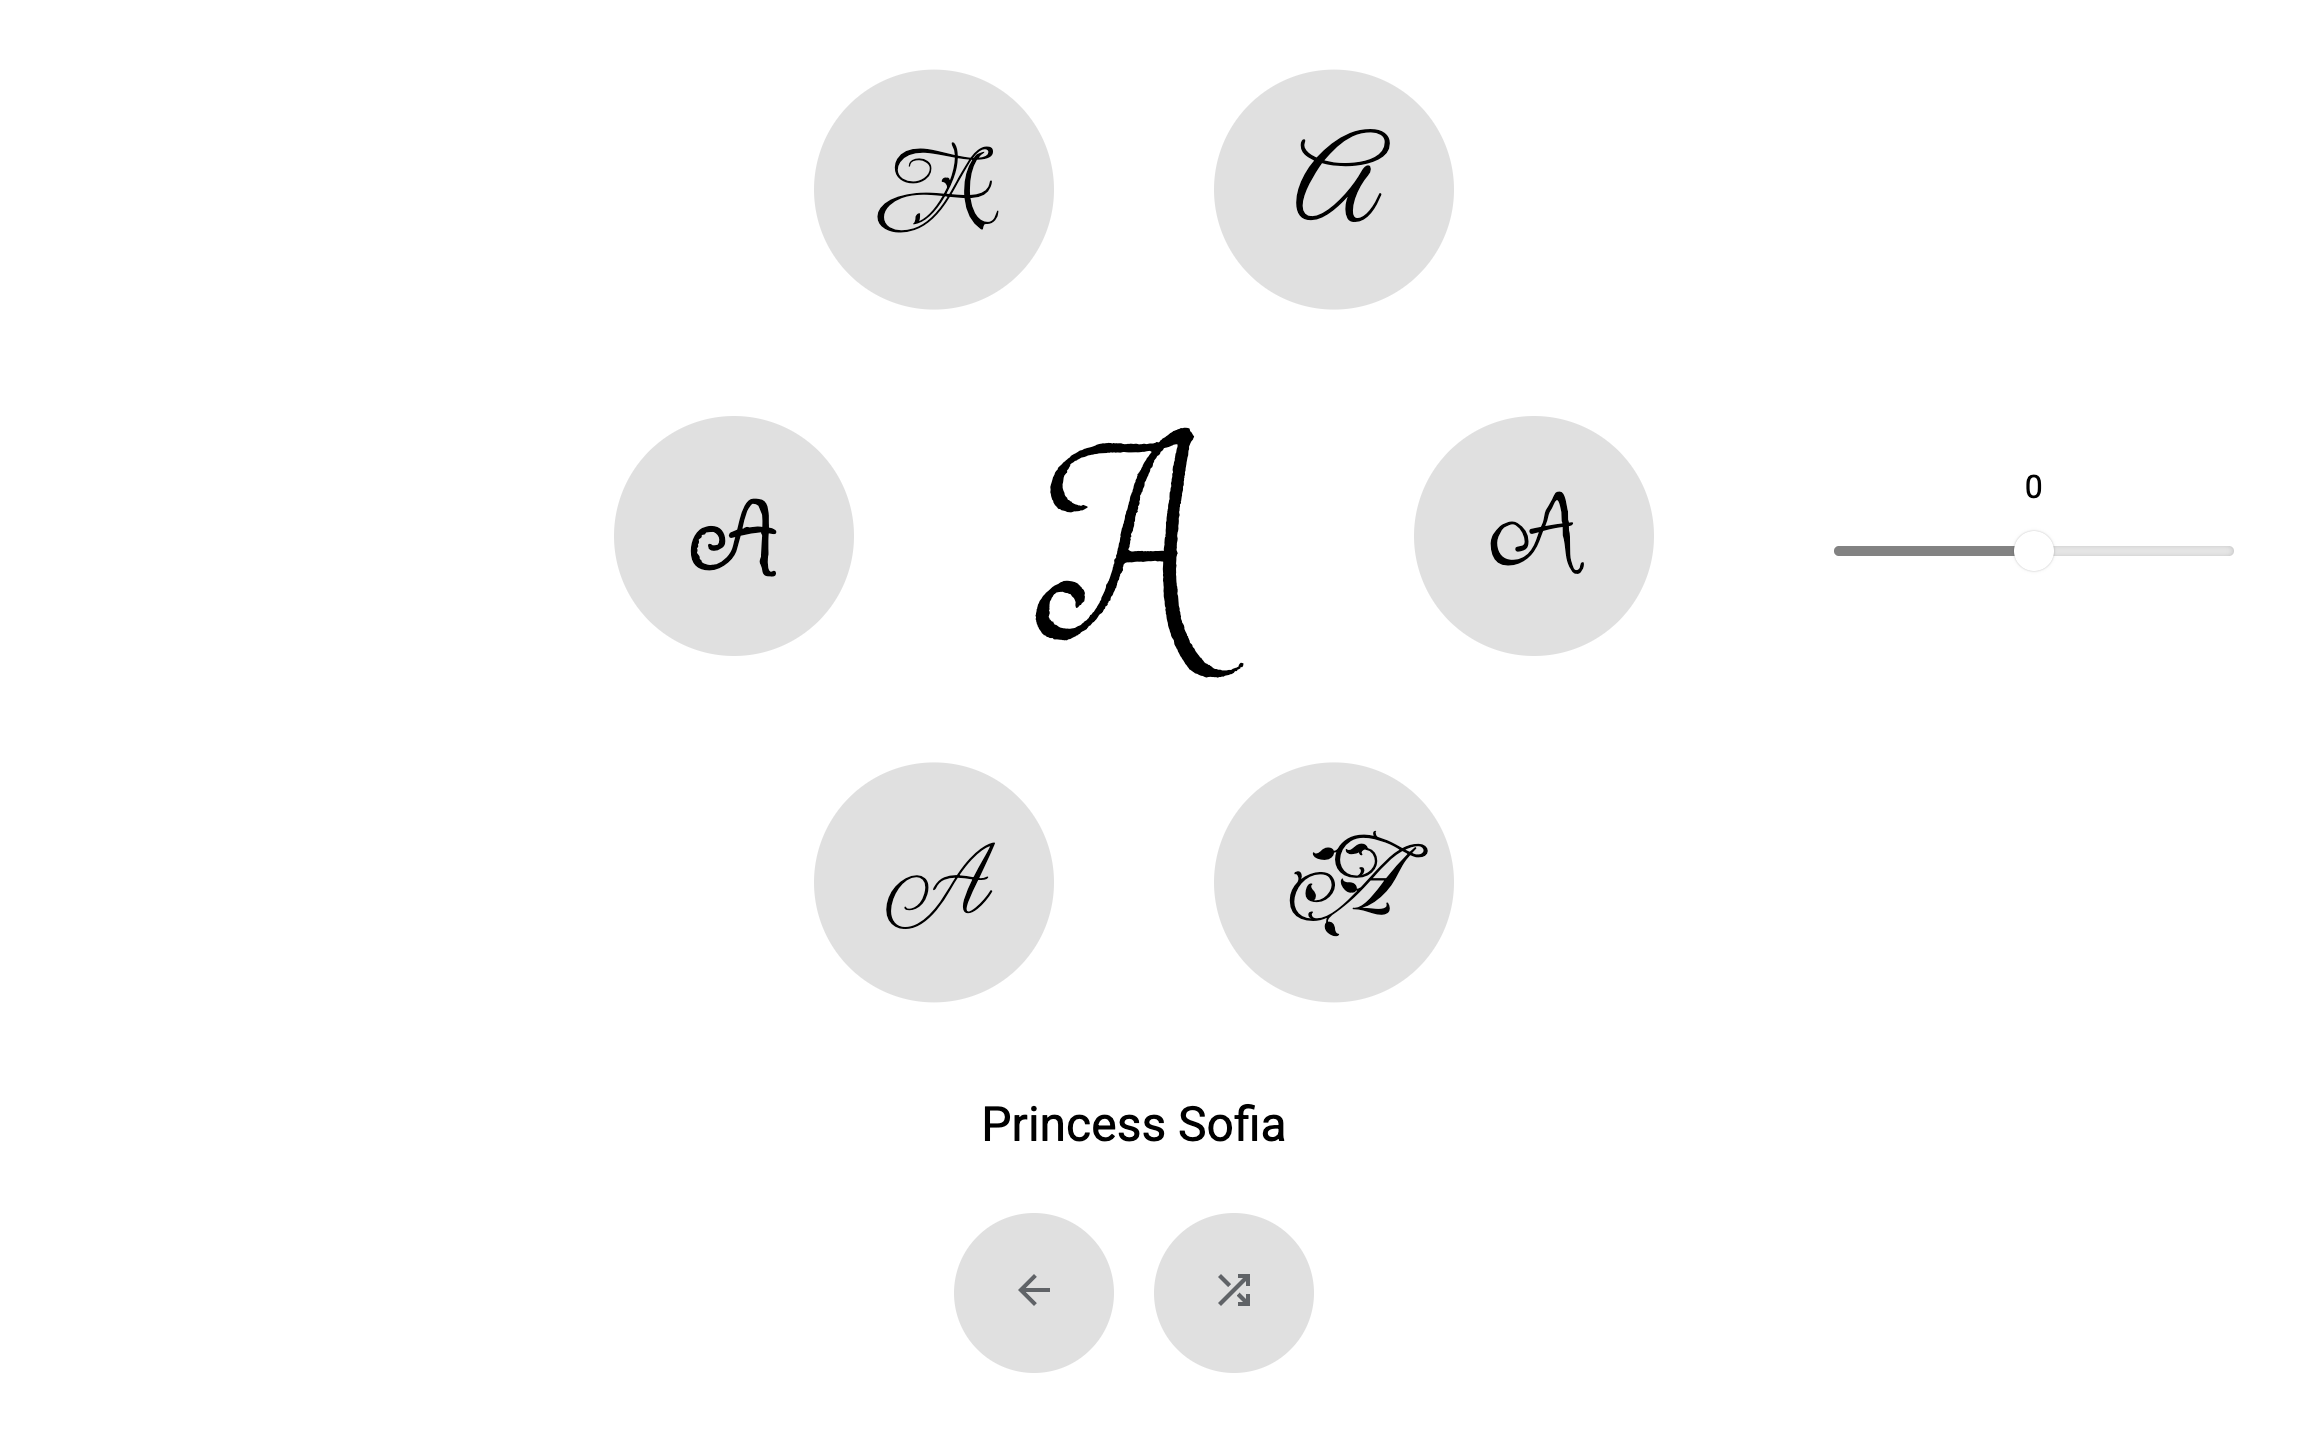
\includegraphics[width=\textwidth]{images/selector-tool.png}
    \caption{Our novel 6-dimensional typeface selector tool, displaying several similar calligraphic fonts nearby the Princess Sofia typeface}
    \label{fig:selector-tool}
\end{figure}

\section{Current Interface}

The current iteration of our typeface selector tool involves two connected components which allow users to explore our 6-dimensional vector style space in complementary ways. The first tool is an interactive scatter plot, displaying a t-SNE reduction of our 6-dimensional style space. t-SNE \cite{vandermaaten2008} is a dimensionality reduction technique, which allows typeface encodings near each other in the original 6-dimensional space to generally remain close to each other in the reduced 2-dimensional space. The scatterplot is an intuitive and familiar representation of spatial data to most users, making it a useful tool for navigating this style-embedding space. Users explore the scatterplot space and visualize the fonts represented at each point; if a user identifies a font with desireable qualities, they are able to find similar fonts by exploring the points nearby.

In order to provide another way for users to interact with this style space—one which preserves the dimensionality of our style encodings and therefore allows users full range over the model space—we include another typeface selector tool based on the 6-dimensional structure of our encoding data. This tool, shown in Figure \ref{fig:selector-tool}, displays a center font glyph (A is the default character, but this can be changed by the user) of a selected typeface in the model space, and shows six alternative typefaces of that font in a circle surrounding it. The slider, on the right hand side, represents magnitude; when the magnitude is zero, the six surrounding fonts represent the nearest neighbors to the center font (determined by Euclidean distance); when the magnitude is nonzero, the tool will search—along all six dimensions of the model space—according to the distance defined by the slider magnitude, and display the closest font in each of those dimensions. Therefore, as the slider grows further from zero, the six fonts displayed will have increasingly different style from the center font. At any point, a user can select one of the six surrounding fonts and move to that point in the model space, at which point the slider resets to zero (nearest neighbor), and the user may continue the process again in order to find a more optimal font. The tool also includes a shuffle button, enabling the user to randomly select a new font, and a back button which allows the user to return to previously seen fonts. By providing easy-to-use buttons and dynamically displaying fonts, this tool enables users to navigate a high-dimensional model space which is difficult to conceptualize intuitively.

% my own figure
\begin{figure}[p]
    \centering
    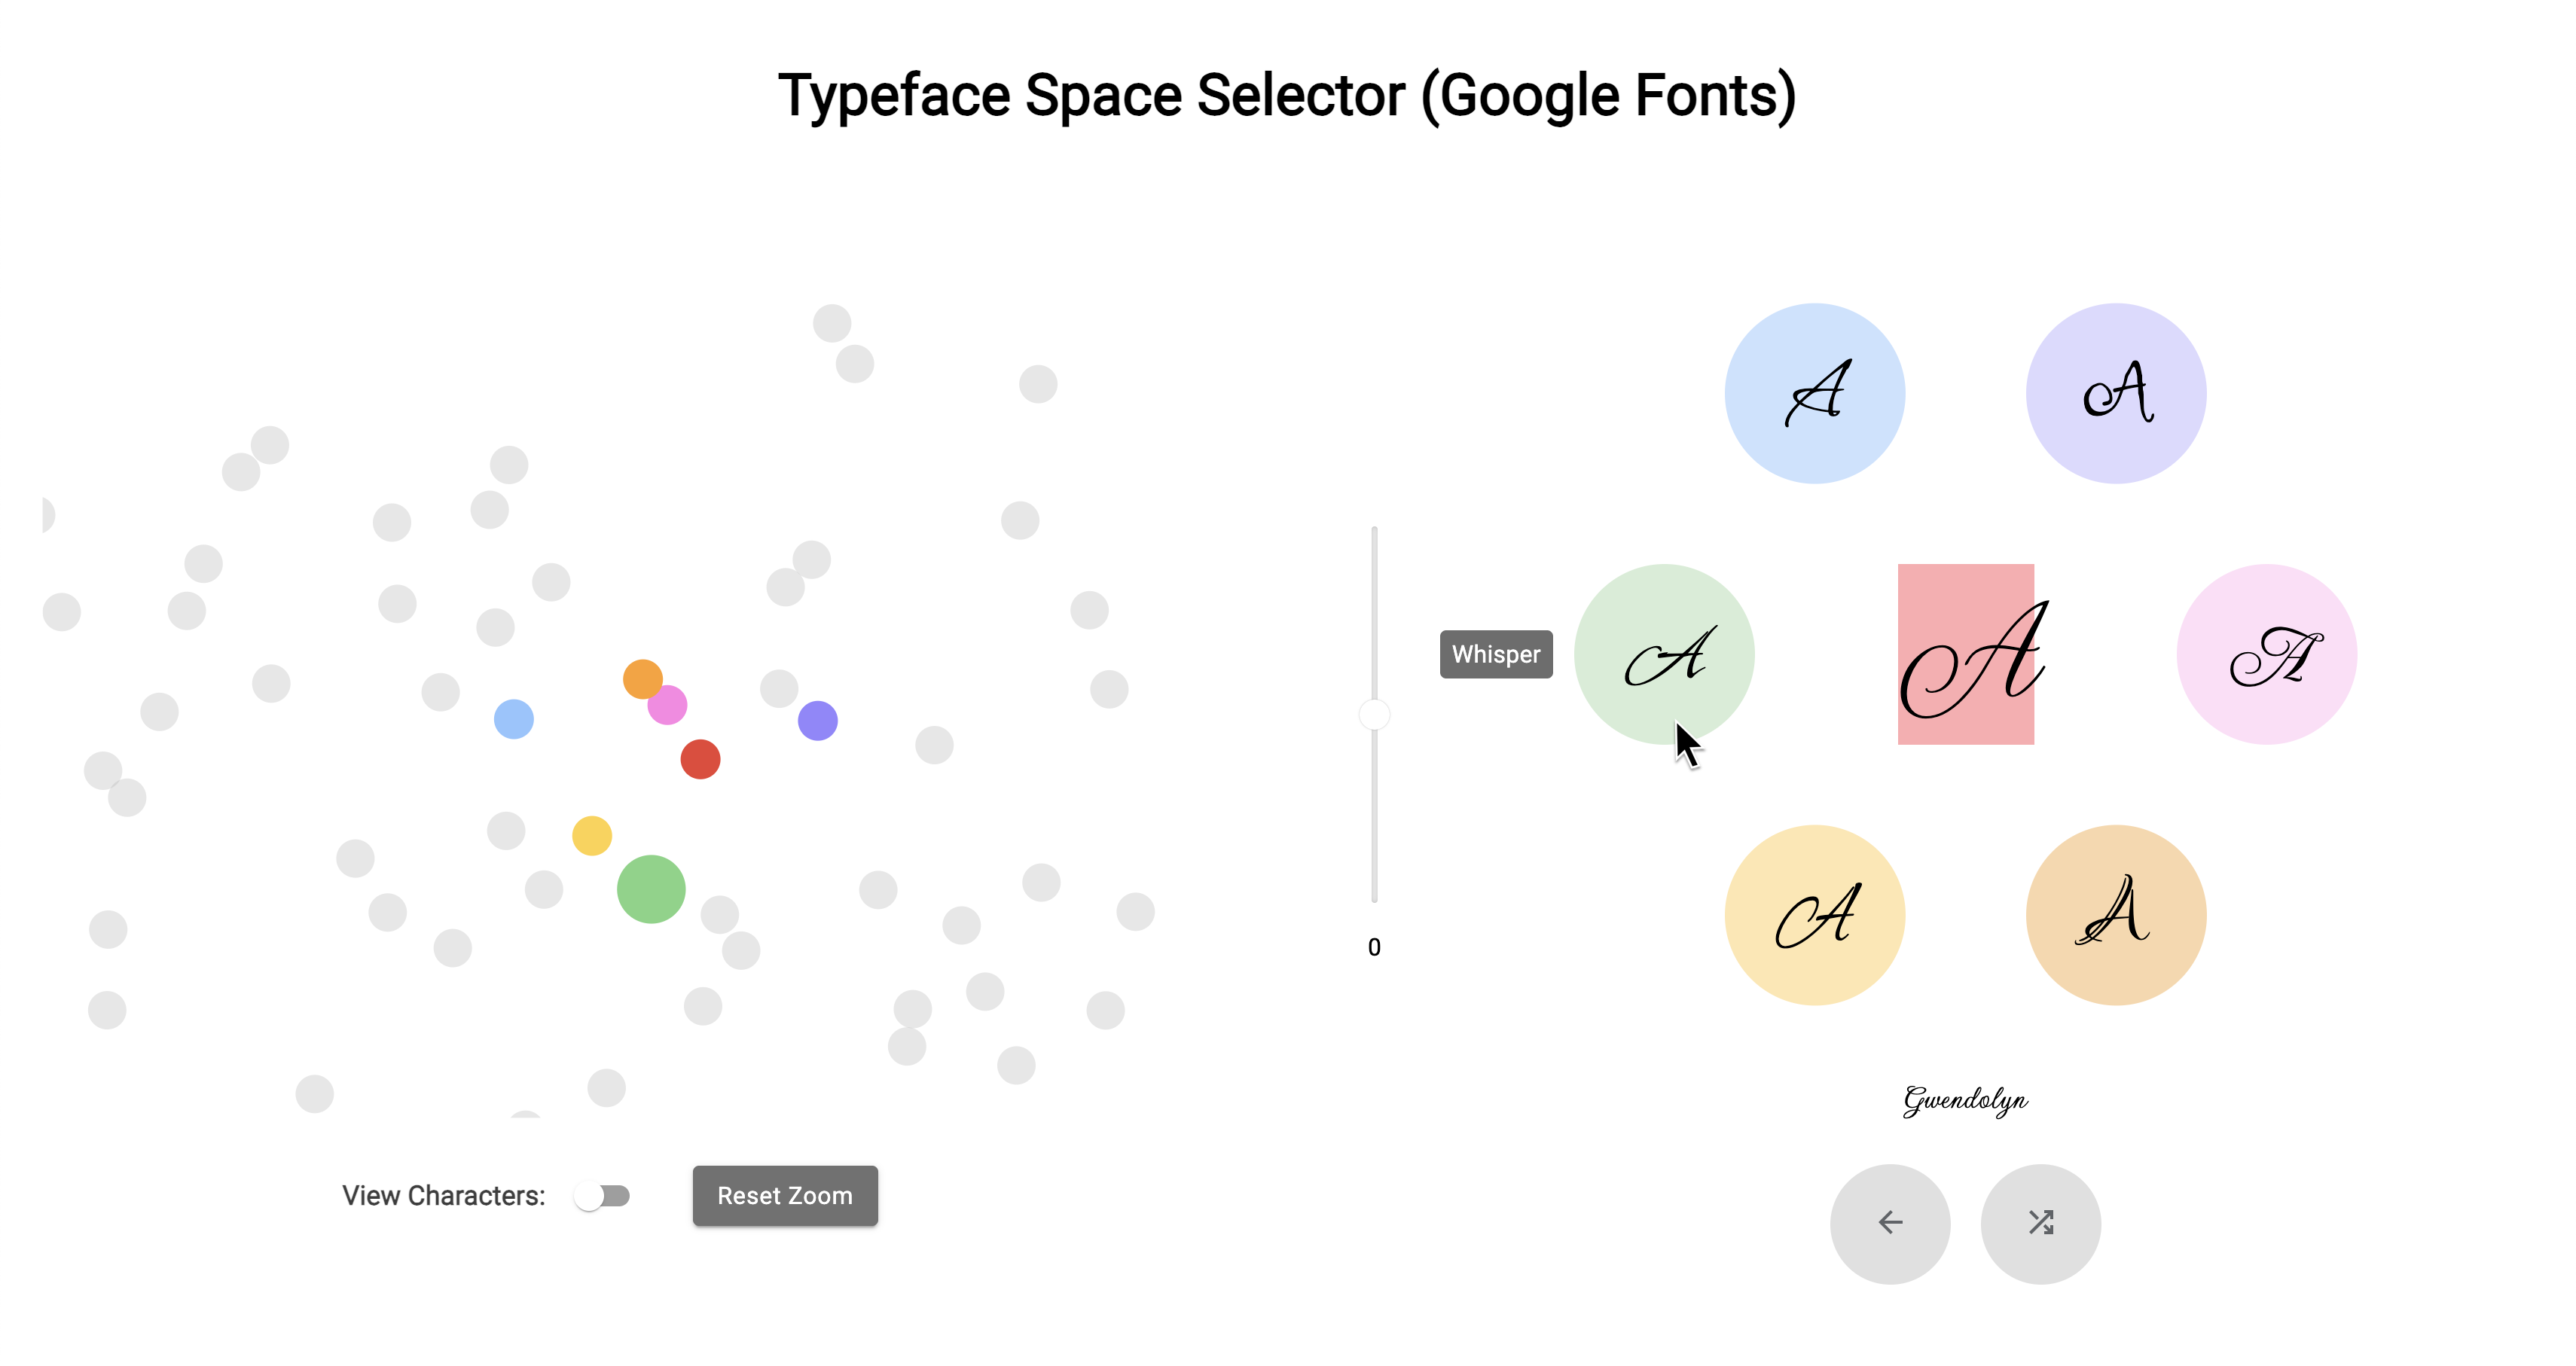
\includegraphics[width=\textwidth]{images/both-selectors.png}
    \caption{Both of our typeface selector tools side-by-side, with additional features to ease use of both tools in tandem}
    \label{fig:both-selectors}
\end{figure}

% my own figure
\begin{figure}[p]
    \centering
    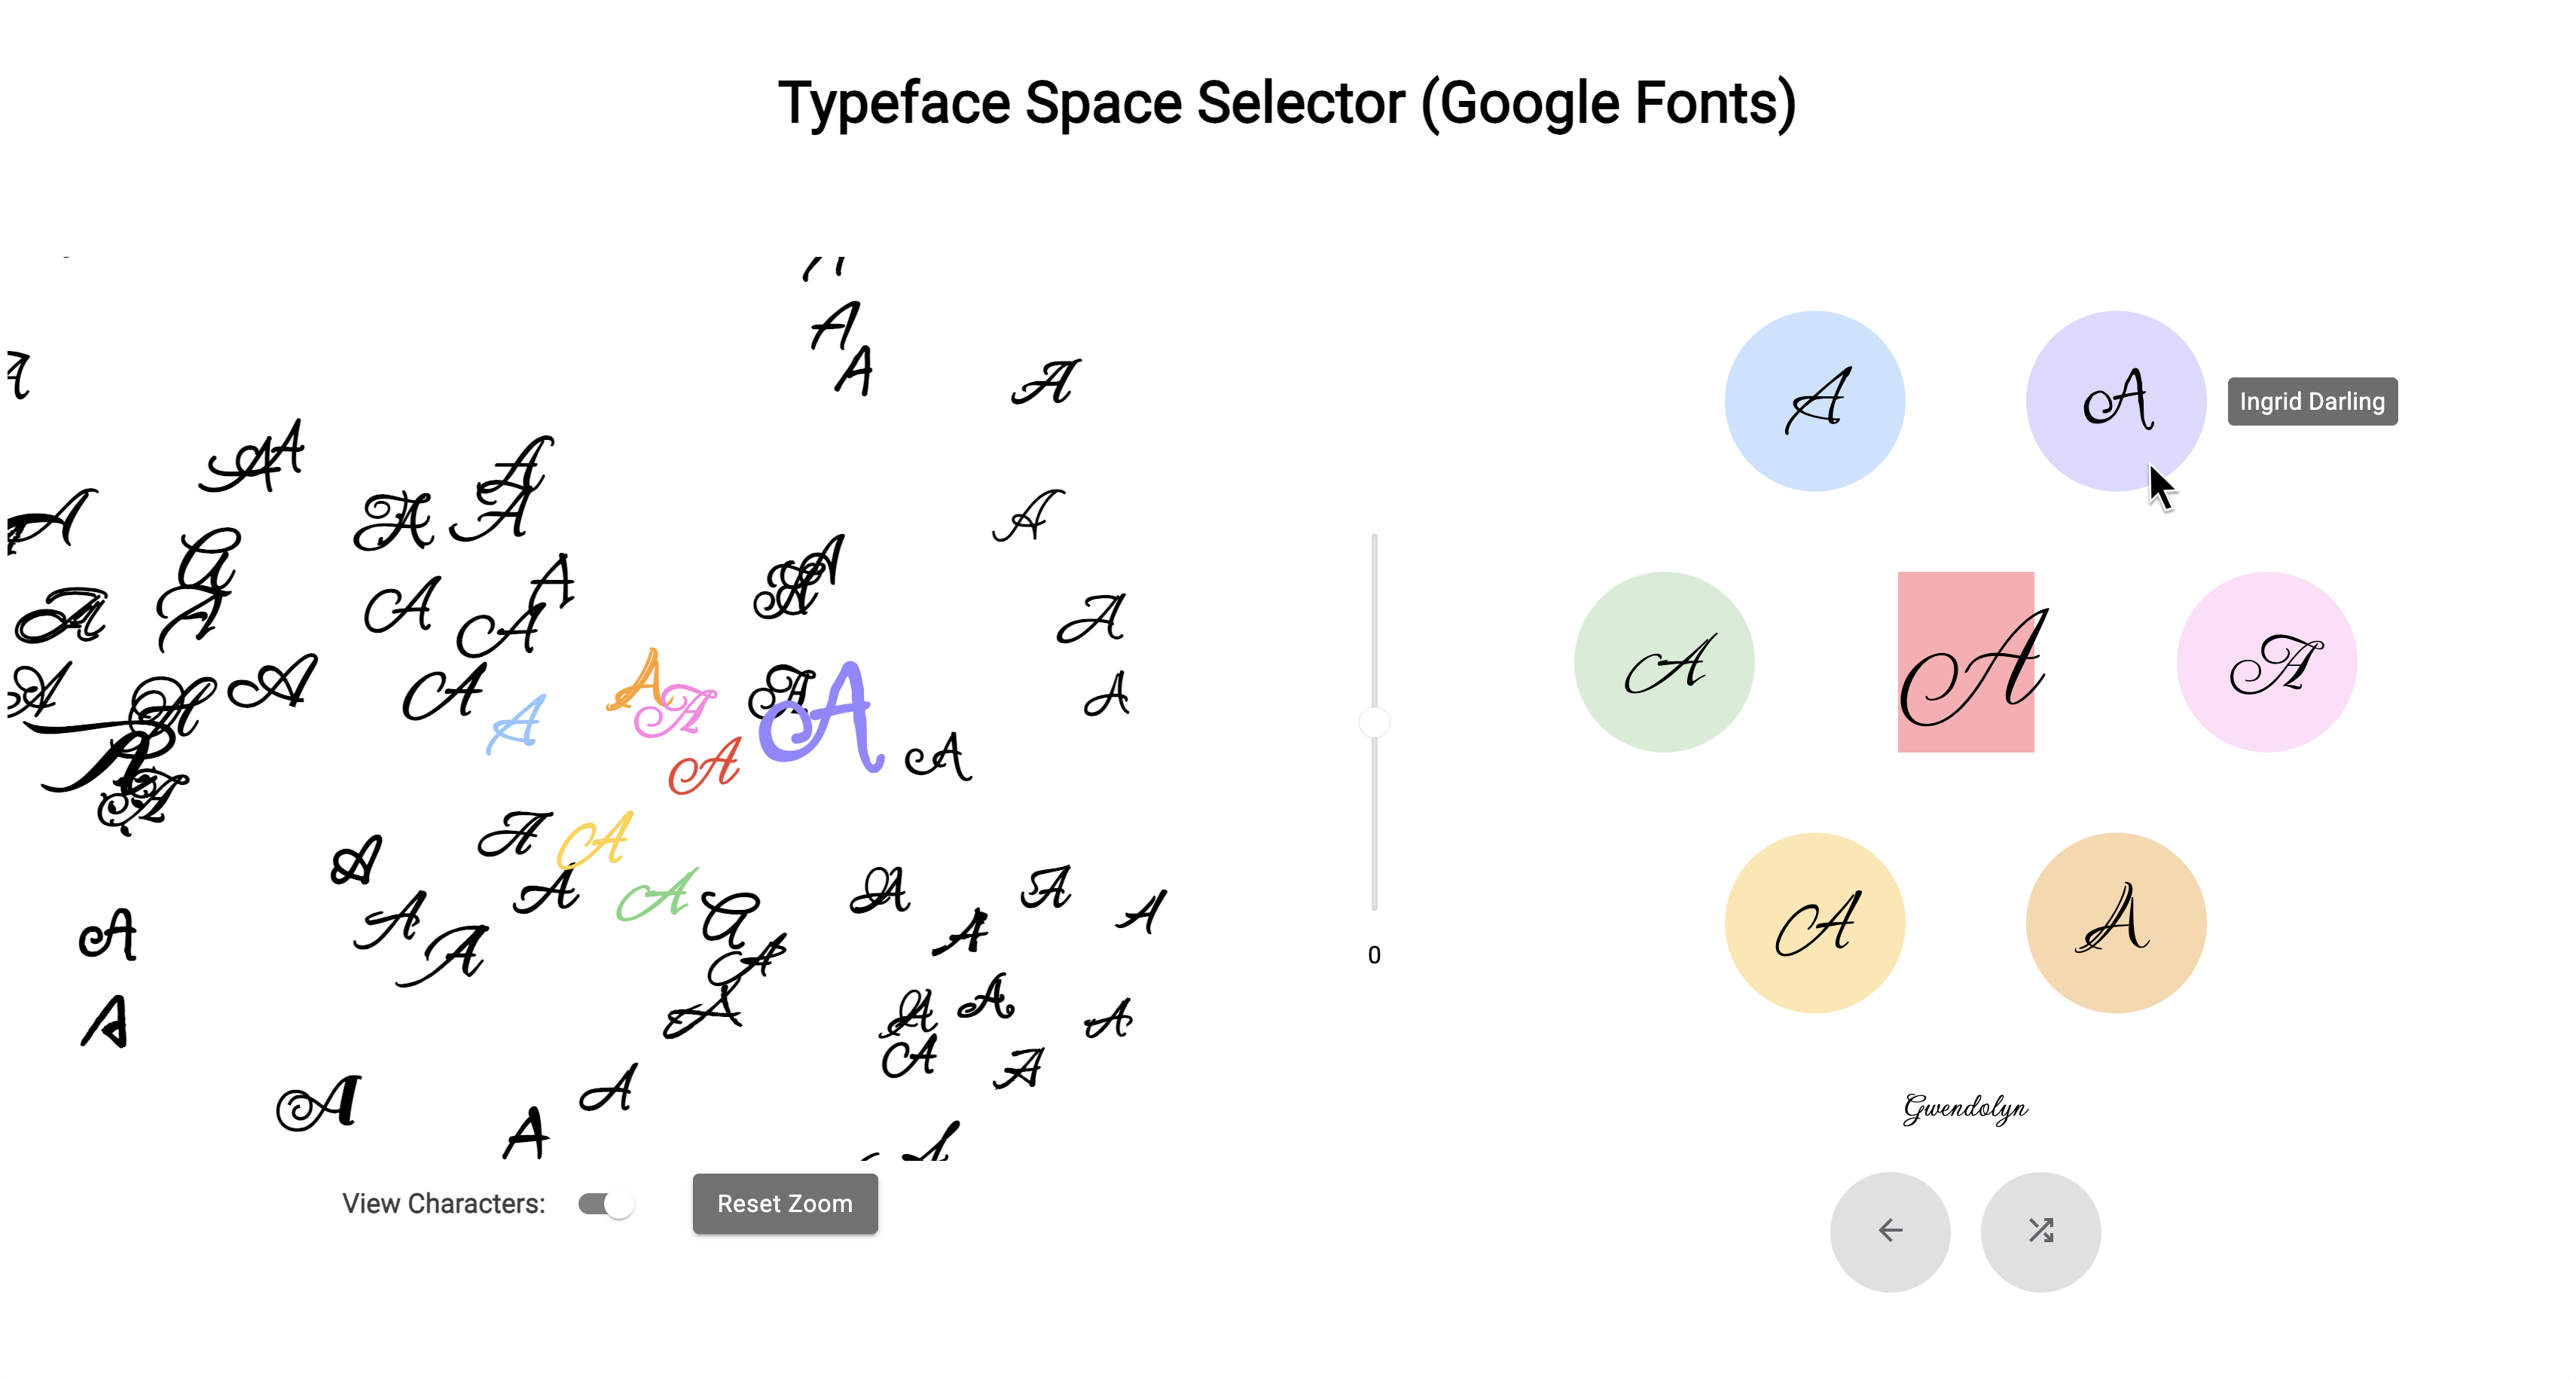
\includegraphics[width=\textwidth]{images/tool-with-chars.png}
    \caption{Our typeface selector tool with characters displayed on scatterplot, showing many nearby calligraphic fonts}
    \label{fig:tool-with-chars}
\end{figure}

Our final product combines both the scatterplot and six-point tool, with several additional features to make the tools work together effectively (see Figure \ref{fig:both-selectors}). Namely, we use distinct colors to display the location of each of the typefaces from the 6-point selector tool within the scatterplot visualization. Additionally, when the cursor hovers over one of the typefaces in the 6-point tool, that point grows bigger in the scatterplot tool, making it even easier and clearer to locate a typeface within the t-SNE scatterplot space. Users click on points in both the scatterplot and the 6-point selector, and the entire tool dynamically updates to the new typeface location. Finally, there is a toggle under the scatterplot to display characters instead of circular points (maintaining colors) which makes for an easier visualization of the entire space, and users zoom and pan around the scatterplot tool to better navigate and explore different areas of the style map (see Figure \ref{fig:tool-with-chars}). Because of the relatively-slow rendering of these fonts, however, displaying characters on the scatterplot does somewhat slow down the zoom capability of the scatterplot.

In order to make our implementation more streamlined, this font selector is currently limited to the Google Fonts collection of typefaces. (This choice is described further in \ref{frontend}.) It would not be too difficult to expand support for fonts outside of the Google Fonts library, however it might require hosting SVG files of the font characters instead of loading full font files---which would become bulky and slow given a large number of fonts. (Consequently, this would likely speed up the tool's performance.) The current implementation of our font selector tool can be found here.\footnote{\url{http://sysnet.cs.williams.edu/~25sm39/}}

\subsection{Backend (Flask)}

We implement the backend of our web app in Flask,\footnote{\url{https://flask.palletsprojects.com/en/stable/}} a lightweight Python web server which adds expanded capability on top of the basic HTTP GET and POST requests and includes support for URL parameters, which we leverage to pass the magnitude data determining the server's nearest neighbors calculations. The backend server provides two functionalities. First, the backend serves the full t-SNE dataset for use in our scatterplot selector tool (a small file <1MB) upon request from the frontend web app. Second, the server is queried to navigate the 6-dimensional model space and compute the nearest neighbor calculations necessary for the six-point font selector tool. Leveraging the Facebook AI Similarity Search (FAISS) library,\footnote{\url{https://ai.meta.com/tools/faiss/}} which provides efficient, high-dimensional vector similarity search, the backend first locates the style encoding for the input typeface, then computes six new style encoding vectors in each of the six dimensions according to the user-specified magnitude. FAISS then finds the nearest actual typeface style encoding for each of the six calculated vectors (see Figure \ref{fig:model-search}) and serves those font names to the client, avoiding duplicates when possible.

% my own figure
\begin{figure}[]
    \centering
    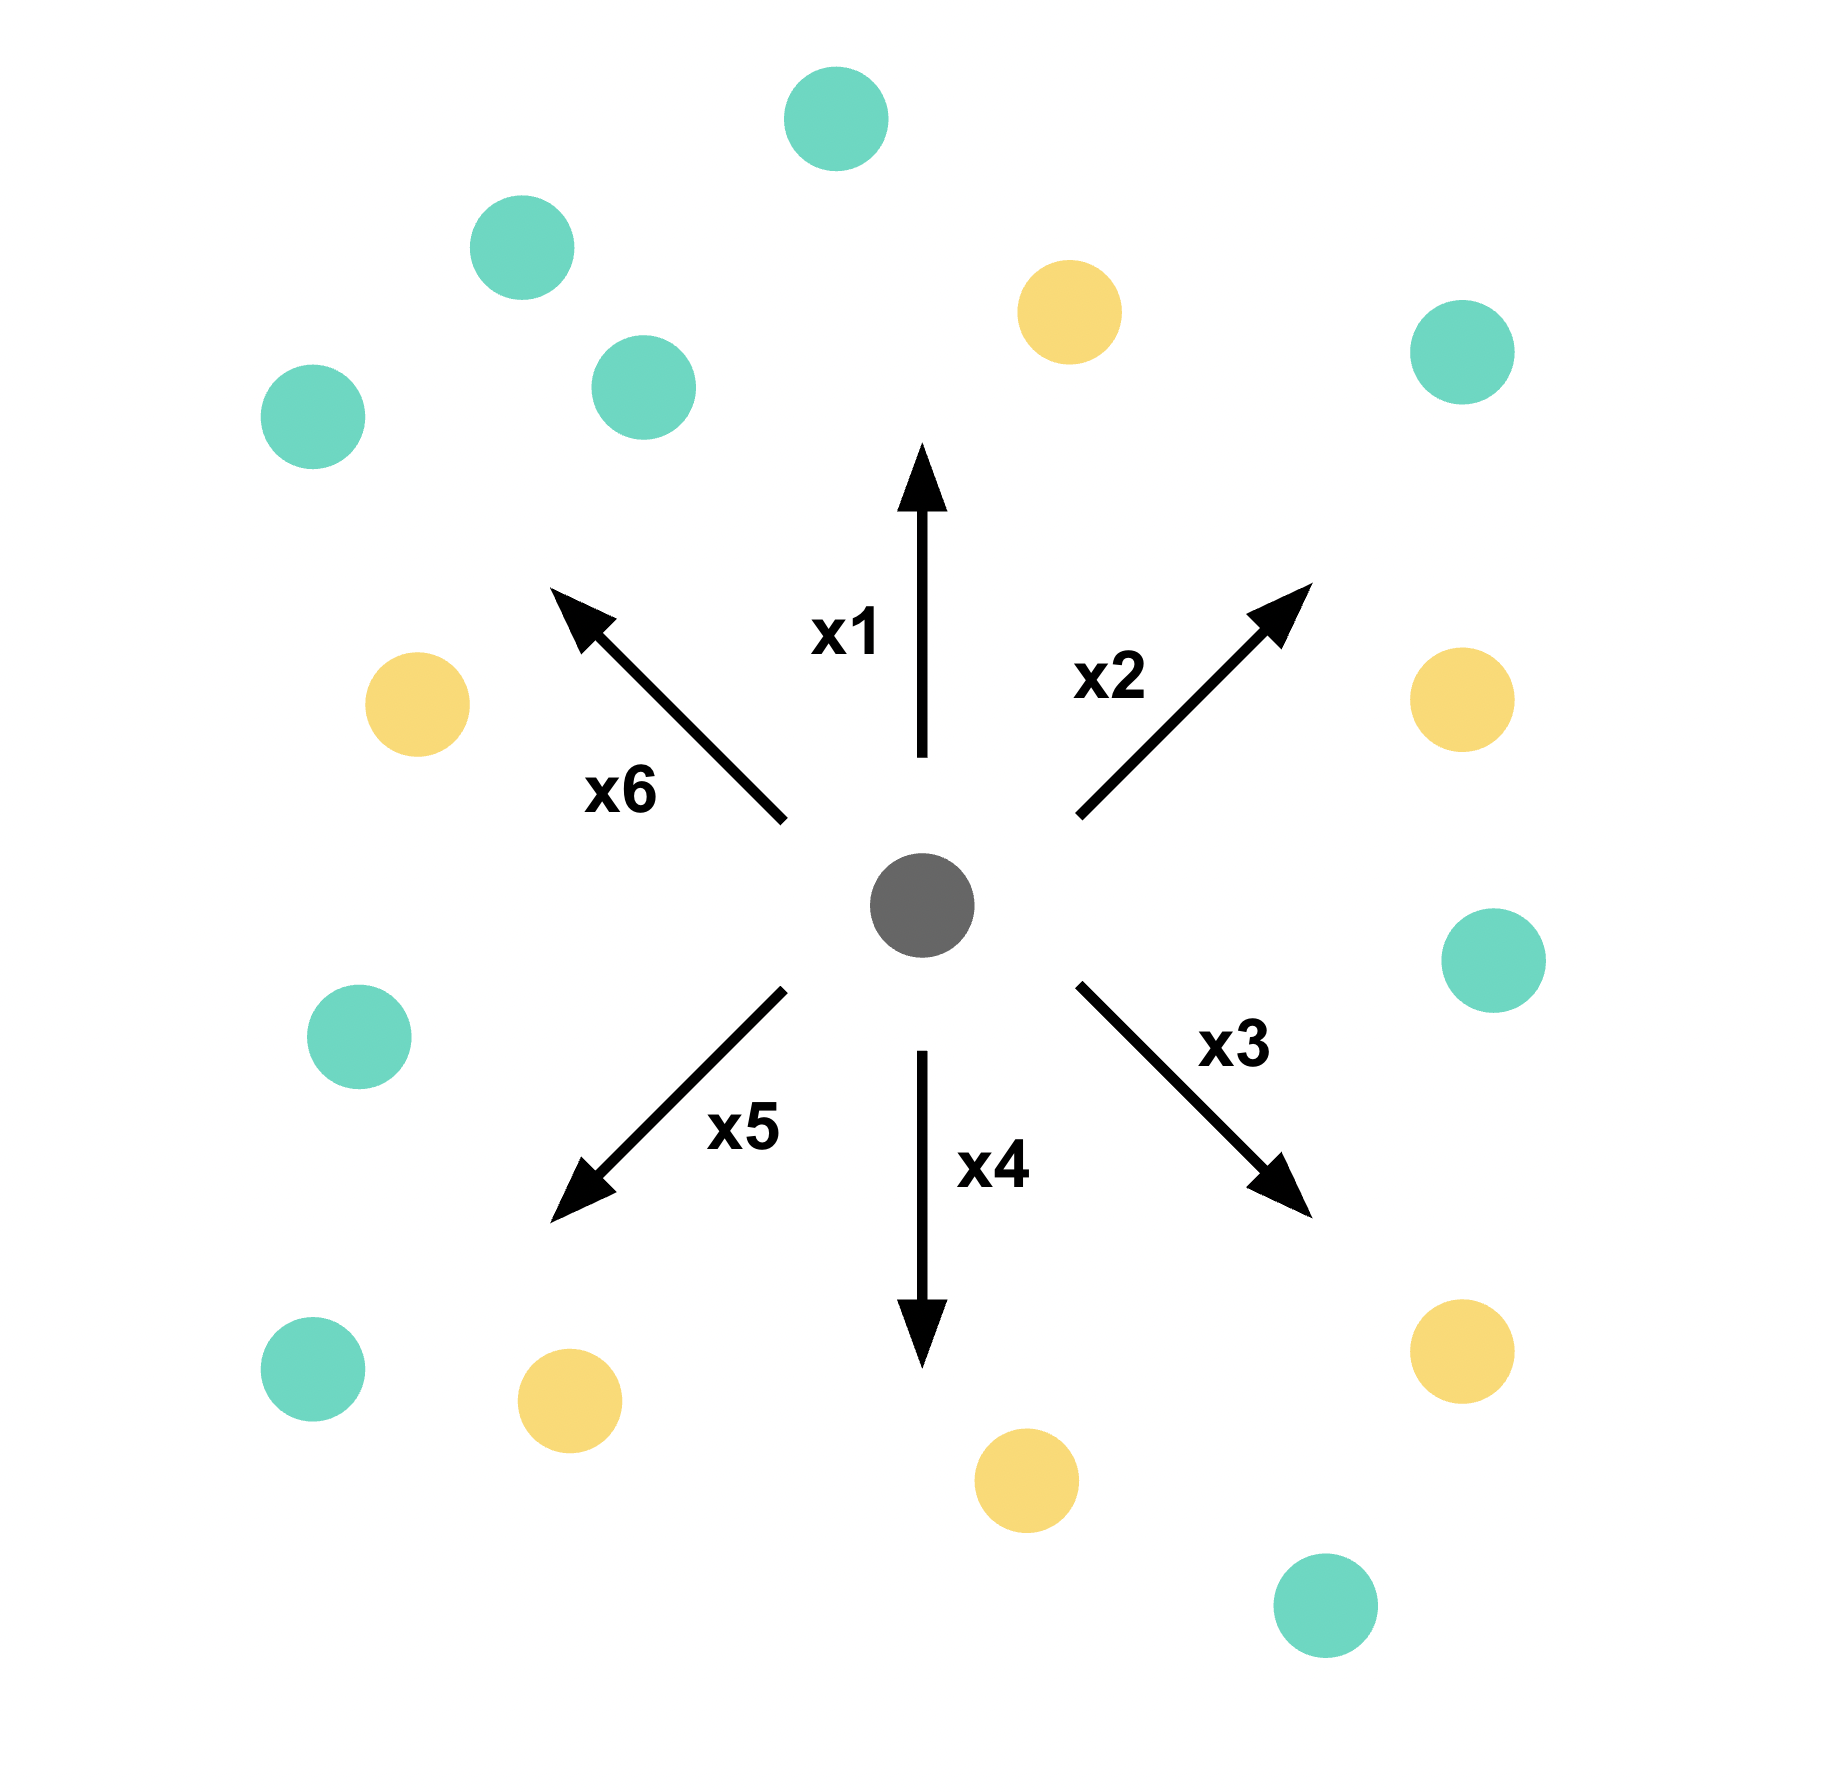
\includegraphics[width=0.62\textwidth]{images/model-search.png}
    \caption{Search algorithm in our model space:\ extend search in each dimension according to magnitude and find nearest neighbor}
    \label{fig:model-search}
\end{figure}

% my own figure
\begin{figure}[]
    \centering
    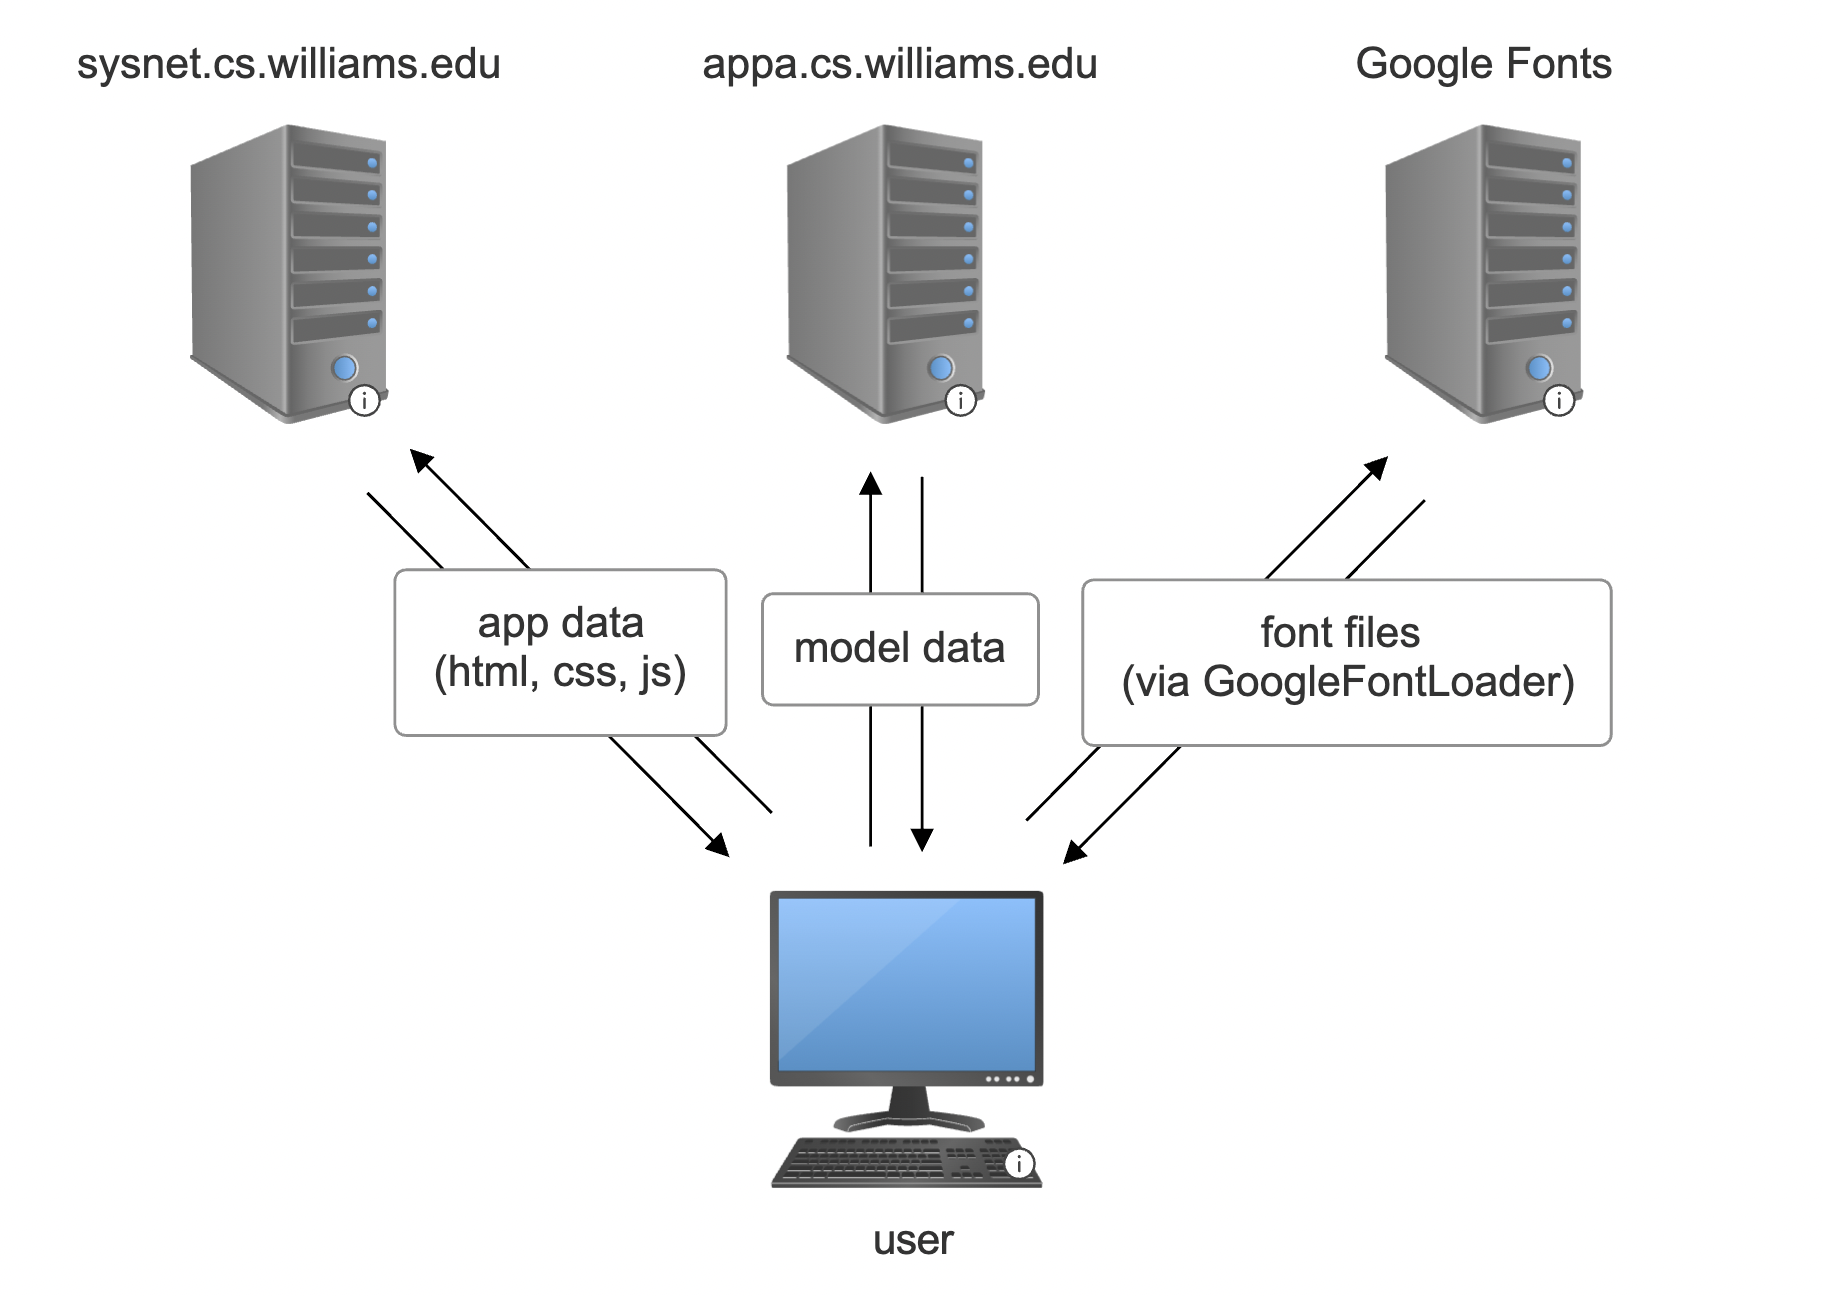
\includegraphics[width=0.9\textwidth]{images/system-diagram.png}
    \caption{A network diagram of our font selector webapp system}
    \label{fig:system-diagram}
\end{figure}

\subsection{Frontend (React)} \label{frontend}

Our frontend is implemented in React,\footnote{\url{https://react.dev/}} an open-source JavaScript library built to create interactive web applications using modular components. The scatterplot tool uses the Chart.js library\footnote{\url{https://www.chartjs.org/}} to facilitate plot creation, and the 6-point font selector was built directly using React components. For rendering the actual font files, our frontend uses the GoogleFontLoader package for React,\footnote{\url{https://www.npmjs.com/package/react-google-font-loader}} which facilitates easy, dynamic font loading on webpages. This allows us to avoid serving the 2.7GB of font binary files, alleviating significant server load; however, it limits our current implementation to typefaces from the Google Fonts library. Although Google Fonts is widely-used and contains a wide range of different fonts, this does mean that common proprietary fonts such as Times New Roman and Comic Sans are not included in the current version of our font selector tool. A diagram of our system architecture can be found in Figure \ref{fig:system-diagram}.

\section{Accessing Code}

The full implementation of this project, including the backend server, the frontend webpage, and the training scripts for the models used to generate these style encodings, can be found in the GitHub repository referenced below.\footnote{\url{https://github.com/Mark-Hopkins-at-Williams/thesis-smagid}}